\chapter{Rappels de Relativité Restreinte}
La première partie de ce chapitre (section 1-4) est constitué exclusivement de rappels de la relativité restreinte. Celle-ci sera importante dans la suite du cours, comme elle reste valable \emph{localement} en présence de gravitation, dans un RLI. La seconde partie du chapitre (section 5-6) approfondit ces notions via une étude de la \emph{structure causale} de l'espace de Minkowski.


\section{Postulats de la relativité restreinte}
En 1905, Einstein énonça les deux postulats de la relativité restreinte:
\begin{theoremframe}
    \begin{post}[Loi de la relativité]
        Les lois de la physique prennent la même forme dans tous les référentiels inertiels. Il est donc impossible de distinguer un référentiel inertiel d'un autre.
    \end{post}
\end{theoremframe}
\begin{theoremframe}
    \begin{post}[Universalité de la vitesse de la lumière]
        La vitesse de la lumière $c$ dans le vide est isotope et prend la même valeur dans tout référentiel inertiel.
    \end{post}
\end{theoremframe}
\section{Définition d'un référentiel inertiel}

La relativité restreinte est une théorie de l'espace-temps plat $\R ^{1,3}$ dont les points sont appelés les événements. Les référentiels permettent d'enregistrer ces événements, et sont composés de:

\begin{enumerate}
    \item un repère spatial cartésien orthonormé au repos de coordonnées $(x, y, z) = x^k$ où $k = 1, 2, 3$
    \item des horloges qui déterminent quand l'événement a lieu $x^0 = ct$. 
\end{enumerate}
Un point $x^\mu\in \R^{1,3}$ dans ce repère avec $\mu=0,1,2,3$ est appelé un quadri-vecteur (ou 4-vecteur), et possède des unités de longueur $[x^\mu ] = L$.
\begin{theoremframe}
\begin{rap}[Principe d'inertie]
    En l'absence de force appliquée, un corps se meut en mouvement rectiligne uniforme ou reste au repos.    
\end{rap}
\end{theoremframe}
\begin{theoremframe}
\begin{defi}
Un \emph{référentiel inertiel} est une référentiel dans lequel le principe d'inertie est vrai. 
\end{defi}
\end{theoremframe}
Un référentiel inertiel est une contrepartie de l'espace euclidien. \footnote{qu'est-ce que cela signifie vraiment contrepartie? Moritz: aucune idée }

Un référentiel non inertiel est par exemple la Terre ou un carrousel qui tourne sur lui-même. En effet dans un carrousel, si une personne envoie une balle à une personne en face de lieu lorsque le carrousel est au repas la balle à une trajectoire en ligne droite ( donc le principe d'inertie est respecter) donc arrive a destination. Alors que quand le carrousel tourne sur lui-même, la personne n'arrivera pas a attraper la balle car elle n'aura pas un mouvement rectiligne (le principe d'inertie n'est pas respecté donc on est pas dans un référentiel inertiel).

\section{Intervalle d'espace-temps}

L'intervalle d'espace-temps plat $\mathcal{M} = \R ^{1,3}$ (avec les coordonnées $x^{\mu}$) est l'objet central de la relativité restreinte. On va voire que l'intervalle d'espace-temps de longueur invariante: $(\Delta s)^2 = \eta _{\mu \nu}\Delta x^{\mu} \Delta x^{\nu} $, est préservé par les transformations de Poincaré propre octocrone $\ISO (3,1)\uparrow$.

L'intervalle d'espace-temps est une contrepartie de la distance euclidienne ($(\Delta r)^2 = (\Delta \vect{x})^2$) sur $\R^{1,3}$.

Soient deux événements $P,Q \in \R^{1,3}$ dont les coordonnées dans un référentiel intertiel $\mathcal{O}$ sont $x_P^{\mu}$ et $x_Q^{\mu}$ séparées par $\Delta x^{\mu}=x^\mu_P-x^\mu_Q$. L'intervalle relativiste est défini par:

\begin{align}
    (\Delta s)^2 &\equiv -(c\Delta t)^2 + (\Delta x)^2 + (\Delta y)^2 + (\Delta z)^2\\
    &= \eta _{\mu \nu} \Delta x^{\mu} \Delta x^{\nu}
\end{align}

où $\eta _{\mu \nu} \equiv \textrm{diag}(-1, 1, 1, 1)$ est la métrique de Minkowski. La sommation est sous-entendue sur les indices répétés. L'intervalle définit une pseudo-métrique sur $\R^{1,3}$: elle n'est pas définie positive, et $d(x^\mu,y^\mu)=0 \centernot \implies x^\mu=y^\mu$.

L'intervalle permet de construire une structure causale sur $\R^{1,3}$: les deux évènements $P$ et $Q$ ont un lien causal si et seulement si $(\Delta s)^2 < 0$. En effet:

\begin{align}
    (\Delta s)^2 > 0 &\implies -(c\Delta t)^2 + (\Delta \vect{x})^2 > 0\\
    &\implies c^2 < \lt \frac{\Delta \vect{x}}{\Delta t} \rt^2 \equiv v^2\\
\end{align}

Mais comme aucune information ne peut propager plus vite que la vitesse,on conclut que les deux évènements ne sont pas en lien causal. 

\begin{theoremframe}
    \begin{propri}
        L'intervalle relativiste est invariant sous changement de référentiel inertiel.
    \end{propri}
\end{theoremframe}
\begin{proof}
    Soient deux événements $P,Q \in \R^{1,3}$ séparés dans un référentiel inertiel $\mathcal{O}$ par des coordonnées $\Delta x^{\mu}$ et dans un référentiel inertiel $\mathcal{O}'$ par des coordonnées $\Delta x'^{\mu}$ .

\begin{center}
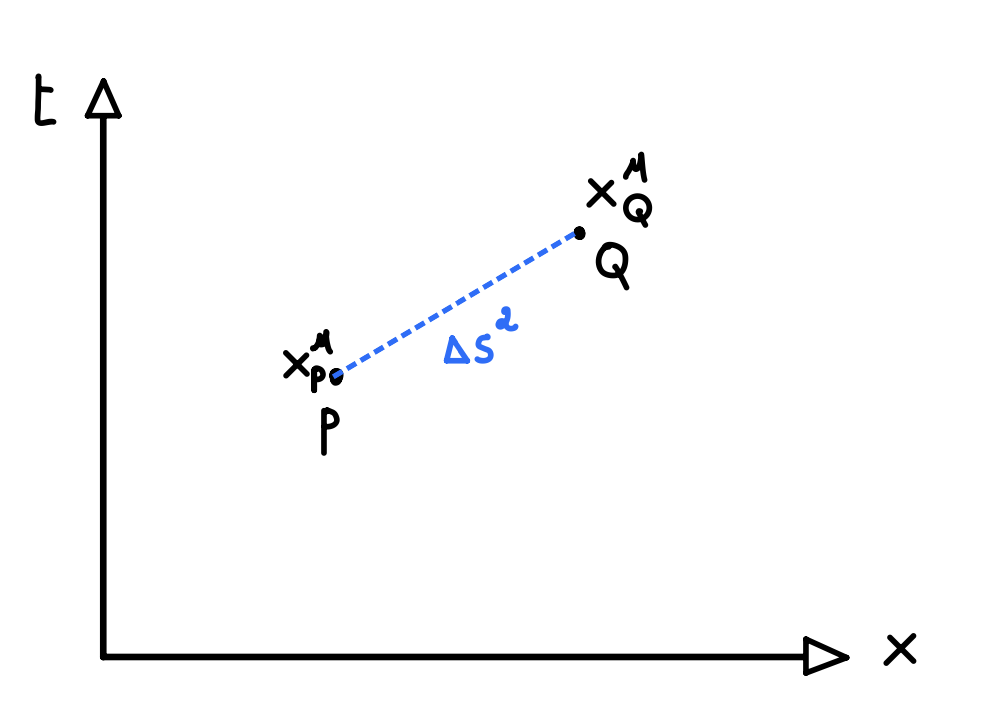
\includegraphics[scale=0.3]{Chapitres/2. Relativité Restreinte/Images/intervalle graph.png}
\end{center}
\begin{enumerate}
    \item Supposons qu'un signal lumineux joigne $P$ à $Q$. On a donc $\lt \dfrac{\Delta \vect{x}}{\Delta t} \rt^2 = v^2 = c^2$. Calculons $(\Delta s )^2$:

\begin{align}
    (\Delta s )^2  & = -(c\Delta t)^2 + (\Delta \vect{x})^2\\
    \lt\frac{\Delta s}{\Delta t}\rt^2 & = -c^2 + \lt \frac{\Delta \vect{x}}{\Delta t} \rt^2\\
    & =0
\end{align}

Ainsi, $\Delta s = 0$. Dans le référentiel $O'$, on aura également $\Delta s' = 0$  car la vitesse de la lumière est la même dans tout les référentiel inertiel.

\begin{equation}
    \lt \frac{\Delta s'}{\Delta t'} \rt^2 = -c^2 + v'^2 = 0
\end{equation}

Il en découle que si l'intervalle s'annule dans un référentiel inertiel, alors il s'annule aussi dans tout référentiel inertiel. 
\item Montrons maintenant que peu importe valeur de $\Delta s$, on a que $\Delta s = \Delta s' $ pour tous référentiels inertiels.

 

Comme les deux référentiels sont inertiels, ils sont reliés par une transformation linéaire: 

\begin{equation}
    x'^{\mu} = \Lambda^{\mu}_{ \; \alpha} x^{\alpha} + a^{\mu}
    \label{def:poincaré}
\end{equation}
où $a\in \R^{1,3}$ est un constante et $\Lambda$ une matrice inversible. Les différences sont alors:

\begin{equation}
    \label{eq:intervalle1}
    \Delta x'^{\mu} = \Lambda^{\mu}_{\alpha} \Delta x^{\alpha}
\end{equation}

et donc l'intervalle dans les deux référentiels s'écrit

\begin{align}
    \label{eq:intervalle2}
    (\Delta s)^2 & = \eta _{\mu \nu} \Delta x^{\mu} \Delta x^{\nu}\\
    \label{eq:intervalle3}
    (\Delta s')^2 & = \eta _{\mu \nu} \Delta x'^{\mu} \Delta x'^{\nu}
\end{align}

et donc $(\Delta s)^2$ et $(\Delta s')^2$ sont deux polynômes du second degré en les $\Delta x^{\mu}$ (comme les $x'^\mu$ dépendent linéairement de $x^\mu$). On a prouvé précédemment que si  $(\Delta s)^2 = 0$ alors   $(\Delta s')^2 = 0$. Les deux polynômes ont donc les mêmes racines. Or deux polynômes du second degré qui ont les mêmes racines sont proportionnelles, c'est-à-dire qu'il existe $\kappa\in \R$ tel que

\begin{equation} 
\label{eq:intervalle4}
(\Delta s)^2 = \kappa (\Delta s')^2.
\end{equation}

L'espace-temps est isotrope donc $\kappa(\vect{v})=\kappa(\lVert \vect{v} \rVert)$\footnote{Etant une propriété des deux référentiels, $\kappa$ ne peut que dépendre $\vect{v}$. Nous invitons le lecteur à argumenter pourquoi celui-ci ne peut pas dépendre des coordonnées d'espace.} et donc en particulier, on trouve $\kappa(\Vec{v}) = \kappa(-\vect{v})$. En effectuant le changement de référentiel inverse, on trouve que

\begin{equation}
    (\Delta s')^2 = \kappa(-\vect{v}) (\Delta s)^2
    \label{eq:intervalle5}
\end{equation}

En combinant\ref{eq:intervalle4} avec \ref{eq:intervalle5}, on obtient finalement

\begin{align}
    (\Delta s)^2 &= \kappa(\vect{v}) \kappa(-\vect{v}) (\Delta s)^2\\
    &= \kappa^2(\Delta s)^2
\end{align}

Il vient que $\kappa ^2= 1$ donc aussi $\kappa = \pm 1$. En injectant \ref{eq:intervalle1} dans \ref{eq:intervalle3}, puis en utilisant la relation \ref{eq:intervalle4}, on trouve que
\begin{equation}
    \eta_{\mu\nu} \Delta x^\mu \Delta x^\nu = \kappa \eta_{\alpha\beta} \Lambda^\alpha_{\; \mu} \Lambda^\beta_{\; \nu}\Delta x^\mu \Delta x^\nu
\end{equation}
soit
\begin{equation}
    \label{eq:Lorentz pre}
    \eta = \kappa\eta'=\kappa \Lambda^T\eta \Lambda
\end{equation}
Comme $\eta$ est une forme quadratique symétrique et $\eta'$ est un changement de base de $\eta$ ($\Lambda$ est inversible), par le \textit{théorème de Sylvester}\footnote{c.f. votre cours d'algèbre de BA1.} que la signature de $\eta'$ ne change pas, et donc que $\kappa=1$.

On peut ainsi conclure que $(\Delta s)^2 = (\Delta s)^2$.
\end{enumerate}
\end{proof}

\section{Transformations de Lorentz et de Poincaré}

On définit les transformations de Poincaré comme l'ensemble des isométries sur l'espace (pseudo-)métrique $(\R^{1,3},s)$, c'est-à-dire les transformations qui relient des référentiels inertiels et telles que la vitesse de la lumière $c$ soit conservée.

Imaginons qu'on a deux référentiels inertiels $O$ et $O'$ qui ont respectivement comme coordonnées $x^{\alpha}$ et $x^{\alpha '}$. 
Comme les deux référentiels sont inertiels ils doivent être reliés par la transformation \ref{def:poincaré}. 

Comme vu dans la section précédente, en prenant $\kappa = 1$ dans la relation \ref{eq:Lorentz pre}, on trouve que

\begin{equation}
    \label{eq:Lorentz}
    \Lambda ^{T} \eta \Lambda = \eta
\end{equation}

L'ensemble des matrices satisfait à l'équation \ref{eq:Lorentz} est appelé le \textit{groupe de Lorentz} O$(3,1)$. L'ensemble des couples $(\Lambda,a)$ satisfaisant à \ref{eq:intervalle1} et donc à \ref{eq:Lorentz} est appelé \textit{groupe de Lorentz inhomogène} ou le \textit{groupe de Poincaré} $IO(3,1)$. 

\begin{rmk}
Lorsque $\eta = \text{diag}(-1,...,-1,1,...,1)$ avec $p$ fois -1 et $q$ fois +1, on appelle le groupe vérifiant \ref{eq:Lorentz} IO$(p,q)$
    
\end{rmk}
\begin{rmk}
    Dans le cas particulier $p =0$ et $q=3$, on a le groupe IO(3) c'est-à-dire avec $\Lambda ^{T} \Lambda = I_{3x3}$. 
\end{rmk}

Les transformations telles que $\Lambda =  I$ appartiennent au groupe de translation.

\subsection{Groupe de Lorentz}

Le groupe de Lorentz O(3,1) possède deux sous-groupes intéressants. En particulier, il possède quatre composantes non-connexes.

\begin{enumerate}
    \item En reprenant la relation $\Lambda ^{T} \eta \Lambda = \eta$, et calculant le déterminant:
    \begin{equation}
        \det \Lambda^{T} \det \eta \det\Lambda = \det \eta \\
        \implies \det\Lambda = \pm 1
    \end{equation}
    Comme il est impossible de passer continument d'un élément de $\det =1$ = un élément de $\det = -1$, le groupe possède deux composantes non-connexes. On note O$(3,1)_\pm$ la partie du groupe de Lorentz à $\det = \pm 1$.\\
    \\
    Uniquement la composante O$(3,1)_+$ est un sous-groupe de O(3,1), appelé groupe spécial de Lorentz noté SO$(3,1)$. \\

    
    \item Réécrivons la relation de définition du groupe de Lorentz. En composantes, on trouve
    \begin{equation}
        \eta_{\alpha \beta} \Lambda_{\;\mu}^{\alpha} \Lambda_{\; \nu}^{\beta} = \eta_{\mu \nu}
    \end{equation}
    Ainsi, pour la composante $\mu = \nu =0$:
    \begin{align}
        \eta_{0 0} &= \eta_{\alpha \beta} \Lambda_{\;0}^{\alpha} \Lambda_{\;0}^{\beta} \\
        \implies -1 &= -(\Lambda_{\;0}^{0})^2 + \sum_{k}(\Lambda_{\;0}^{k})^2\\
        \implies (\Lambda_{\;0}^{0})^2 &= 1 + \sum_{k}(\Lambda_{\;0}^{k})^2\\
        \implies (\Lambda_{\;0}^{0})^2 &\geq 1
    \end{align}
    On trouve donc de nouveau deux composantes non connexes notées O(3,1)$^\uparrow$ (si $\Lambda_{\;0}^{0} \geq 1$) et O(3,1)$^\downarrow$ (si $\Lambda_{\;0}^{0} \leq - 1$). Uniquement O(3,1)$^\uparrow$ est un sous-groupe de O(3,1) et est aussi appelé le sous-groupe orthochrone de Lorentz.
\end{enumerate}
Le groupe O(3,1)$^\uparrow_+ =$ SO(3,1)$^\uparrow$ est un sous-groupe normal de O(3,1). Nous renvoyons vers votre cours de théorie des groupes pour une étude en profondeur du groupe de Lorentz.
\subsection{Exemple de transformation de Lorentz:}

\begin{exmp}
    Une rotation autour de l'axe $z$ peut être décrite par la matrice
    \begin{equation}
        \Lambda = \begin{pmatrix}
1 & 0 & 0 & 0\\
0 & \cos{\theta} & \sin{\theta} & 0\\
0 & -\sin{\theta} & \cos{\theta} & 0\\
0 & 0 & 0 & 1\\
\end{pmatrix}
    \end{equation}
    En notant $x'=\Lambda x$, on peut réécrire cette transformation comme
    \begin{align}
    \left\{
\begin{array}{l}
  t' =t \\
  x' = x\cos{\theta} + y\sin{\theta}\\
  y' = -x\sin{\theta} + y\cos{\theta}\\
  z' = z
\end{array}
\right.
\end{align}
Correspondant bien à une rotation autour de $z$.
\end{exmp}


\begin{exmp}
    Un \textit{boost} dans la direction $x$ peut être décrite par la matrice
    \begin{equation}
        \Lambda = \begin{pmatrix}
\cosh{\phi}& -\sinh{\phi} & 0 & 0\\
-\sinh{\phi} & \cosh{\phi} & 0 & 0\\
0 & 0 & 1 & 0\\
0 & 0 & 0 & 1\\
\end{pmatrix}
    \end{equation}
    De nouveau, on peut réécrire cette transformation comme 
\begin{align}
\label{eq:4.2.1}
    \left\{
\begin{array}{l}
  t' = \cosh{\phi}t - \sinh{\phi}x \\
  x' = -\sinh{\phi}t + \cosh{\phi}x\\
  y' = y\\
  z' = z
\end{array}
\right.
\end{align}
\end{exmp}
Pour montrer que cette transformation correspond bien à un boost dans la direction $x$, nous allons effectuer un changement de variable qui nous ramène aux transformations de Lorentz sous leur forme usuelle.

Posons $-1 < v\deq\tanh\phi < 1$ . Définissons de plus $\gamma \deq \cosh\phi$. Alors, $\sinh\phi = v \gamma$ et la transformation \ref{eq:4.2.1} se réécris comme
\begin{align}
\left\{
\begin{array}{l}
  t' = \gamma(t - vx) \\
  x' = \gamma(x - vt)\\
  y' = y \\
  z' = z
\end{array}
\right.
\end{align}
On peut également montrer que $\gamma$ correspond au facteur de Lorentz usuel:
\begin{align}
    \cosh^2{\phi} - \sinh^2{\phi} = 1\\
    \implies  1 - \tanh{\phi}^2 = \frac{1}{\cosh^2{\phi}}
\intertext{Donc}
    1 - v^2 = \frac{1}{\cosh^2{\phi}}
\intertext{Soit}
    \gamma = \sqrt{\frac{1}{1-v^2}} = \cosh{\phi}
\end{align}

\section{Structure causale de l'espace-temps de Minkowski}

\subsection{Le cône de lumière}
On introduit la notion de cône de lumière. 
\begin{theoremframe}
    \begin{defi}
        Soit $P \in \mathcal{M} = \R^{1, 3} = \mathcal{M}^{1, 3}$. Le \textit{cône de lumière} de $P$, noté $C_P$ est l'ensemble des points à distance nulle de $P$.
        \begin{equation}
            C_P = \ltc Q \in \mathcal{M} \mid \Delta s_{PQ} = 0\rtc
        \end{equation}

    \end{defi}
\end{theoremframe}
On se rappelle que l'intervalle d'espace-temps peut se réécrire comme:
\begin{equation}
    (\Delta s)^2 = -(\Delta t)^2 + \sum_{i}(\Delta x^{i})^2
\end{equation}
Le faite que $(\Delta s)^2 = 0$ implique donc que $\Delta t =
\sqrt{(\Delta x)^2 + (\Delta y)^2 + (\Delta z)^2}$, qui est la contrainte d'un 4-cône (à tout temps $\Delta t$ fixe, il s'agit d'une sphère de rayon $\Delta t$).

\begin{theoremframe}
    \begin{notat}
        Le cône de lumière va diviser l'espace de Minkowski en 3 régions tel que:
        \begin{enumerate}
            \item[\cRM{1}.] \textit{Le futur absolu} de $P$ correspond au cône de lumière supérieur rempli noté $C_{P}^{+}$.
            \item[\cRM{2}.] \textit{Le passé absolu} de $P$ correspond au cône de lumière inférieur rempli noté $C_{P}^{-}$. 
            \item[\cRM{3}.] \textit{L'ailleurs absolu} de $P$ correspond au complémentaire de $C_P^\pm $.
        \end{enumerate}
    \end{notat}
\end{theoremframe}
Ces trois régions sont illustrés sur la figure \ref{fig:2.1}. Justifions cette terminologie. Soient $P,Q\in \R^{1,3}$.

\begin{theoremframe}
    \begin{propri}
         Si $Q \in C_P^+$ (resp. $C_P^-$), alors $Q$ se produit après (resp. avant) $P$ pour tout référentiel inertiel.
    \end{propri}
\end{theoremframe}
\begin{proof}
    Exercice.
\end{proof}
La causalité est importante dans une théorie physique. Cette propriété assure que la causalité de deux évènements causalement connectés (ils se trouvent dans le cône de lumière de l'autre) est conservée pour tout référentiel inertiel. 
    \begin{figure}[H]
     \centering
        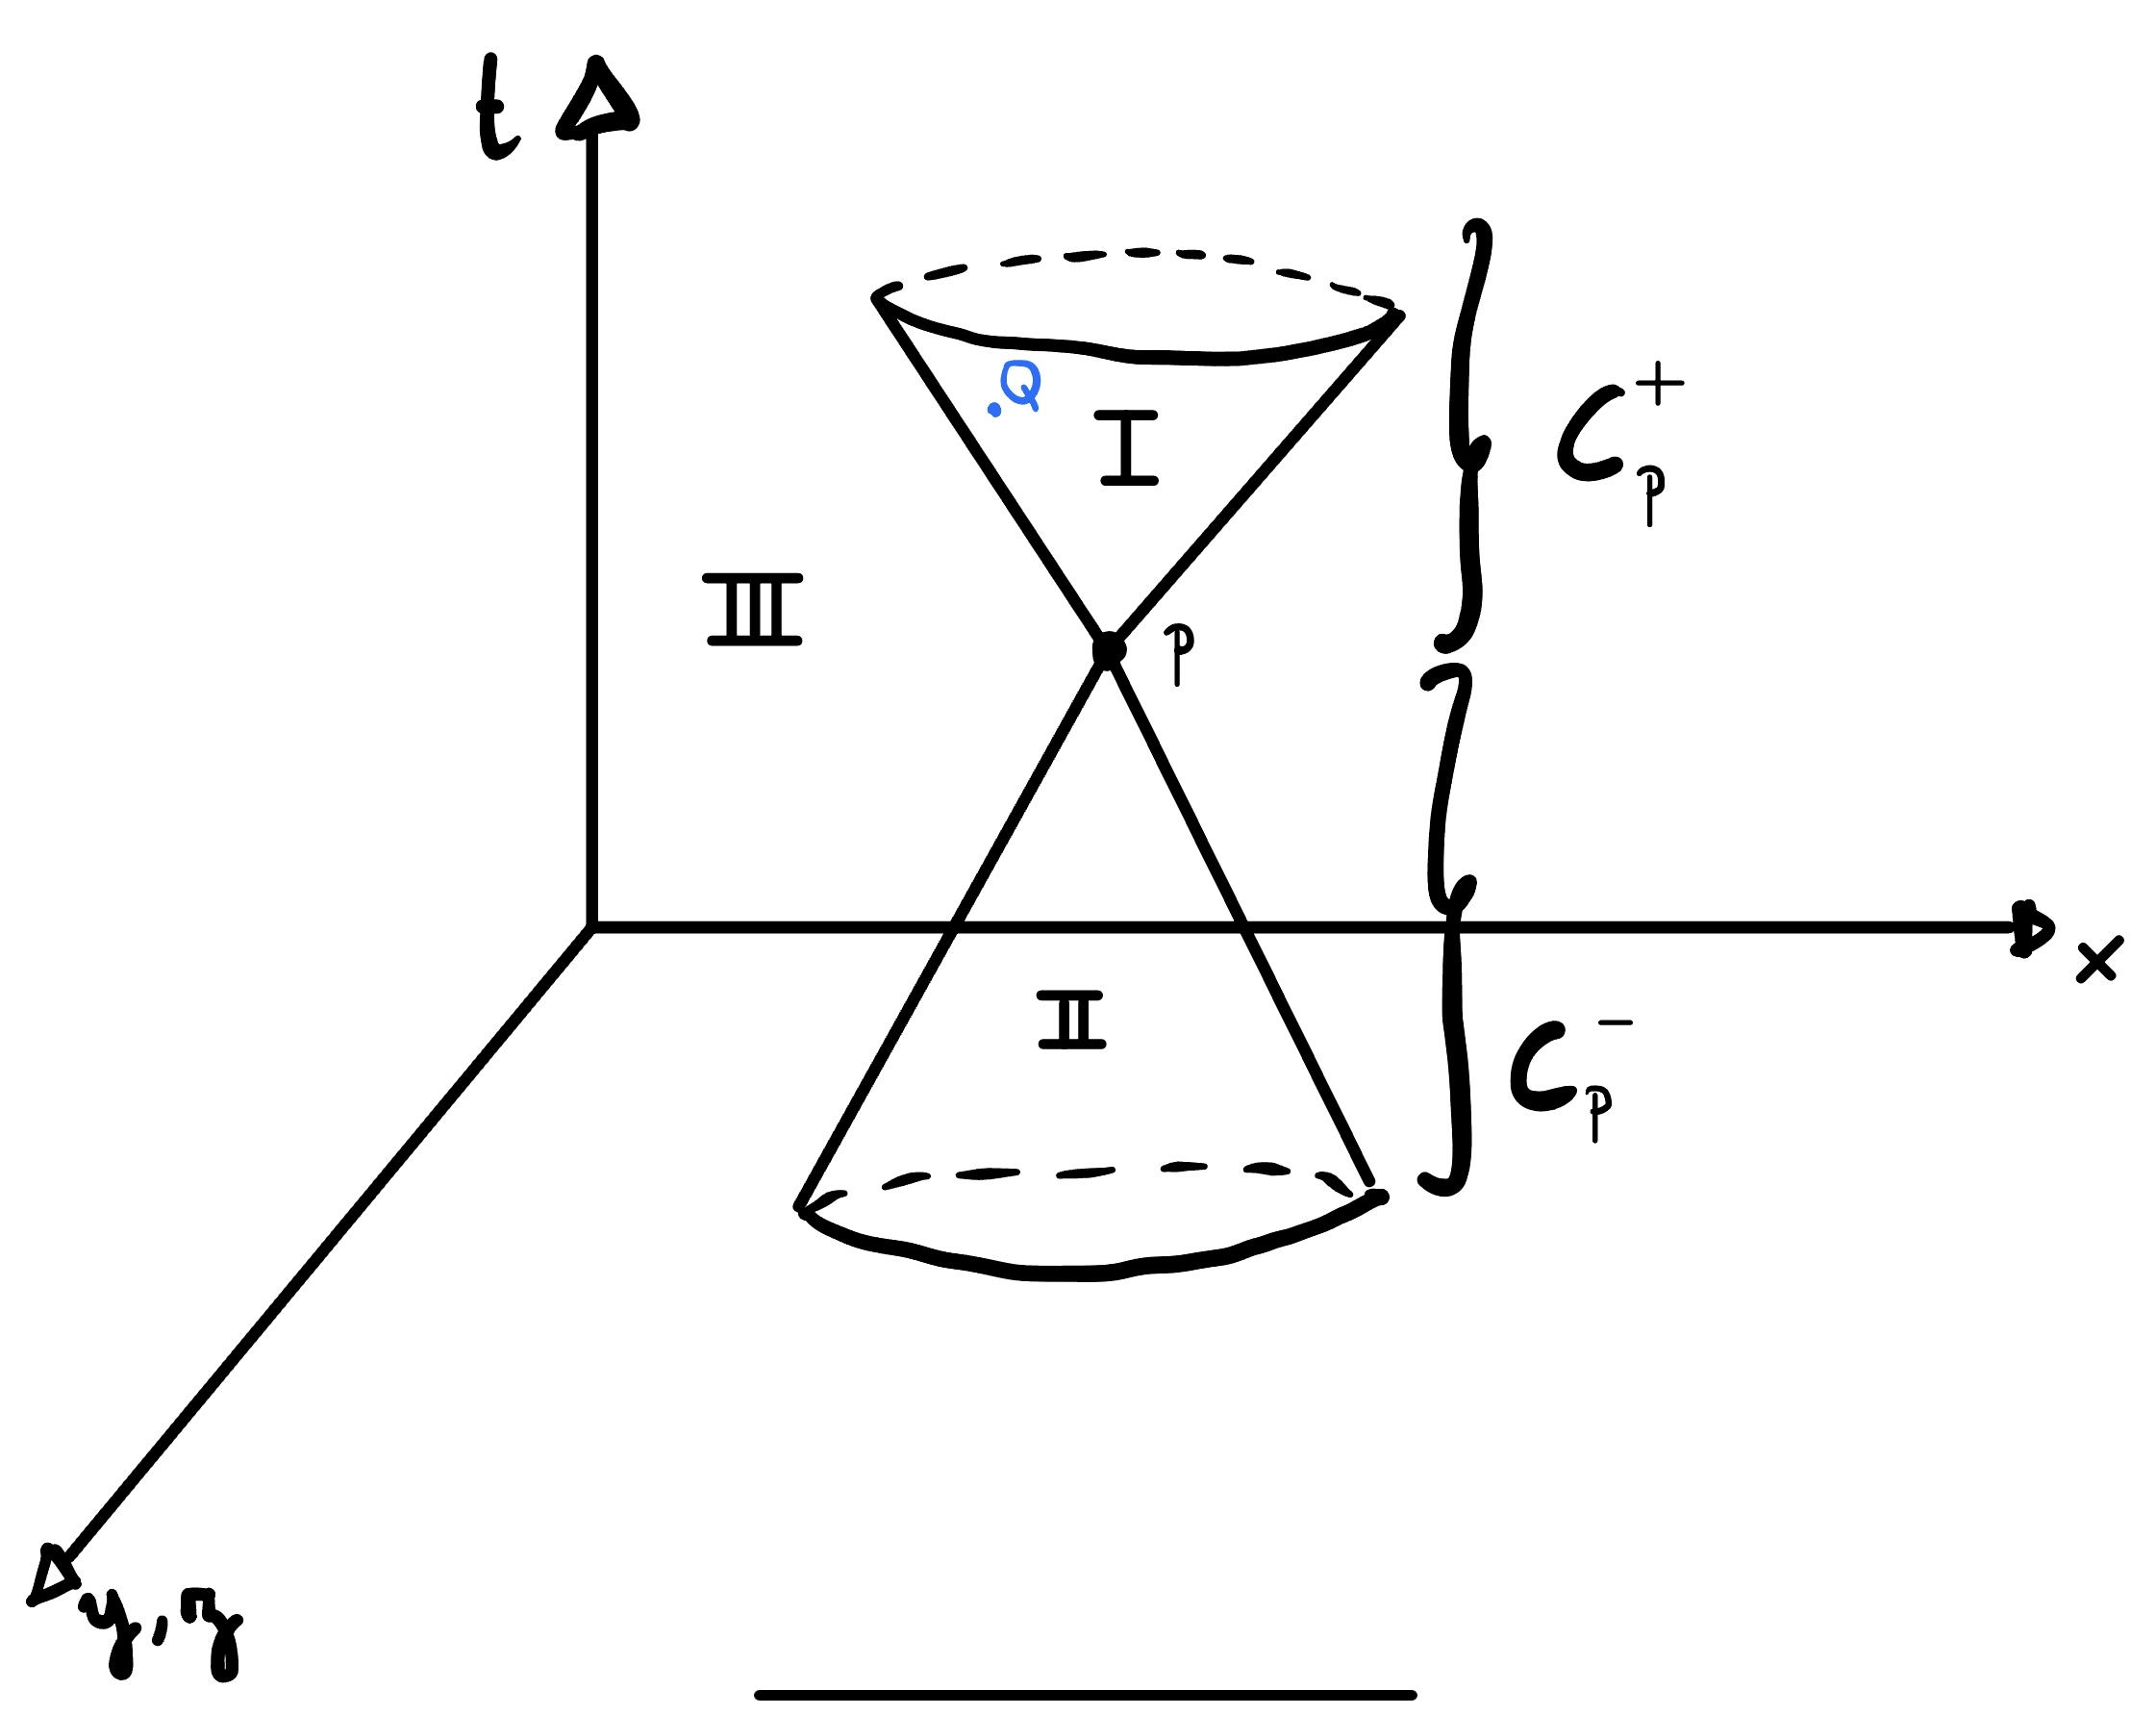
\includegraphics[width=0.5\textwidth]{Chapitres/2. Relativité Restreinte/Images/Cone de lumière avec point Q dans 1.jpg}
        \caption{Le cône de lumière de $P$ représenté dans l'espace $\R^{1,2}$}
        \label{fig:2.1}
\end{figure}

\begin{theoremframe}
    \begin{propri}
        Si $(\Delta s)^2_{PQ} < 0$ alors on peut trouver un référentiel inertiel pour lequel $P$ et $Q$ se passent au même endroit c'est-à-dire que $\Delta x^{i}_{PQ }= 0$.
    \end{propri}
\end{theoremframe}
\begin{proof}
    Exercice.
\end{proof}
    Comme on est dans le cas où $(\Delta s)^2_{PQ} < 0$ (intérieur du cône), $P$ et $Q$ sont en contact causal. Graphiquement, la propriété précédente est facile à démontrer, comme le montre la figure \ref{fig:2.2}. En effet, comme $Q$ se trouve à l'intérieur du cône de lumière de $P$, et en se rappelant de l'effet d'un boost sur les axes du nouveau référentiel $O'$, il est possible de trouver un référentiel dont l'axe de temps $t'$ relie $P$ à $Q$. Ainsi, $\Delta x = 0$. Il est en revanche impossible de trouver un référentiel inertiel dans lequel les deux évènements ont lieu en même temps.
\begin{figure}[H]
    \begin{center}
        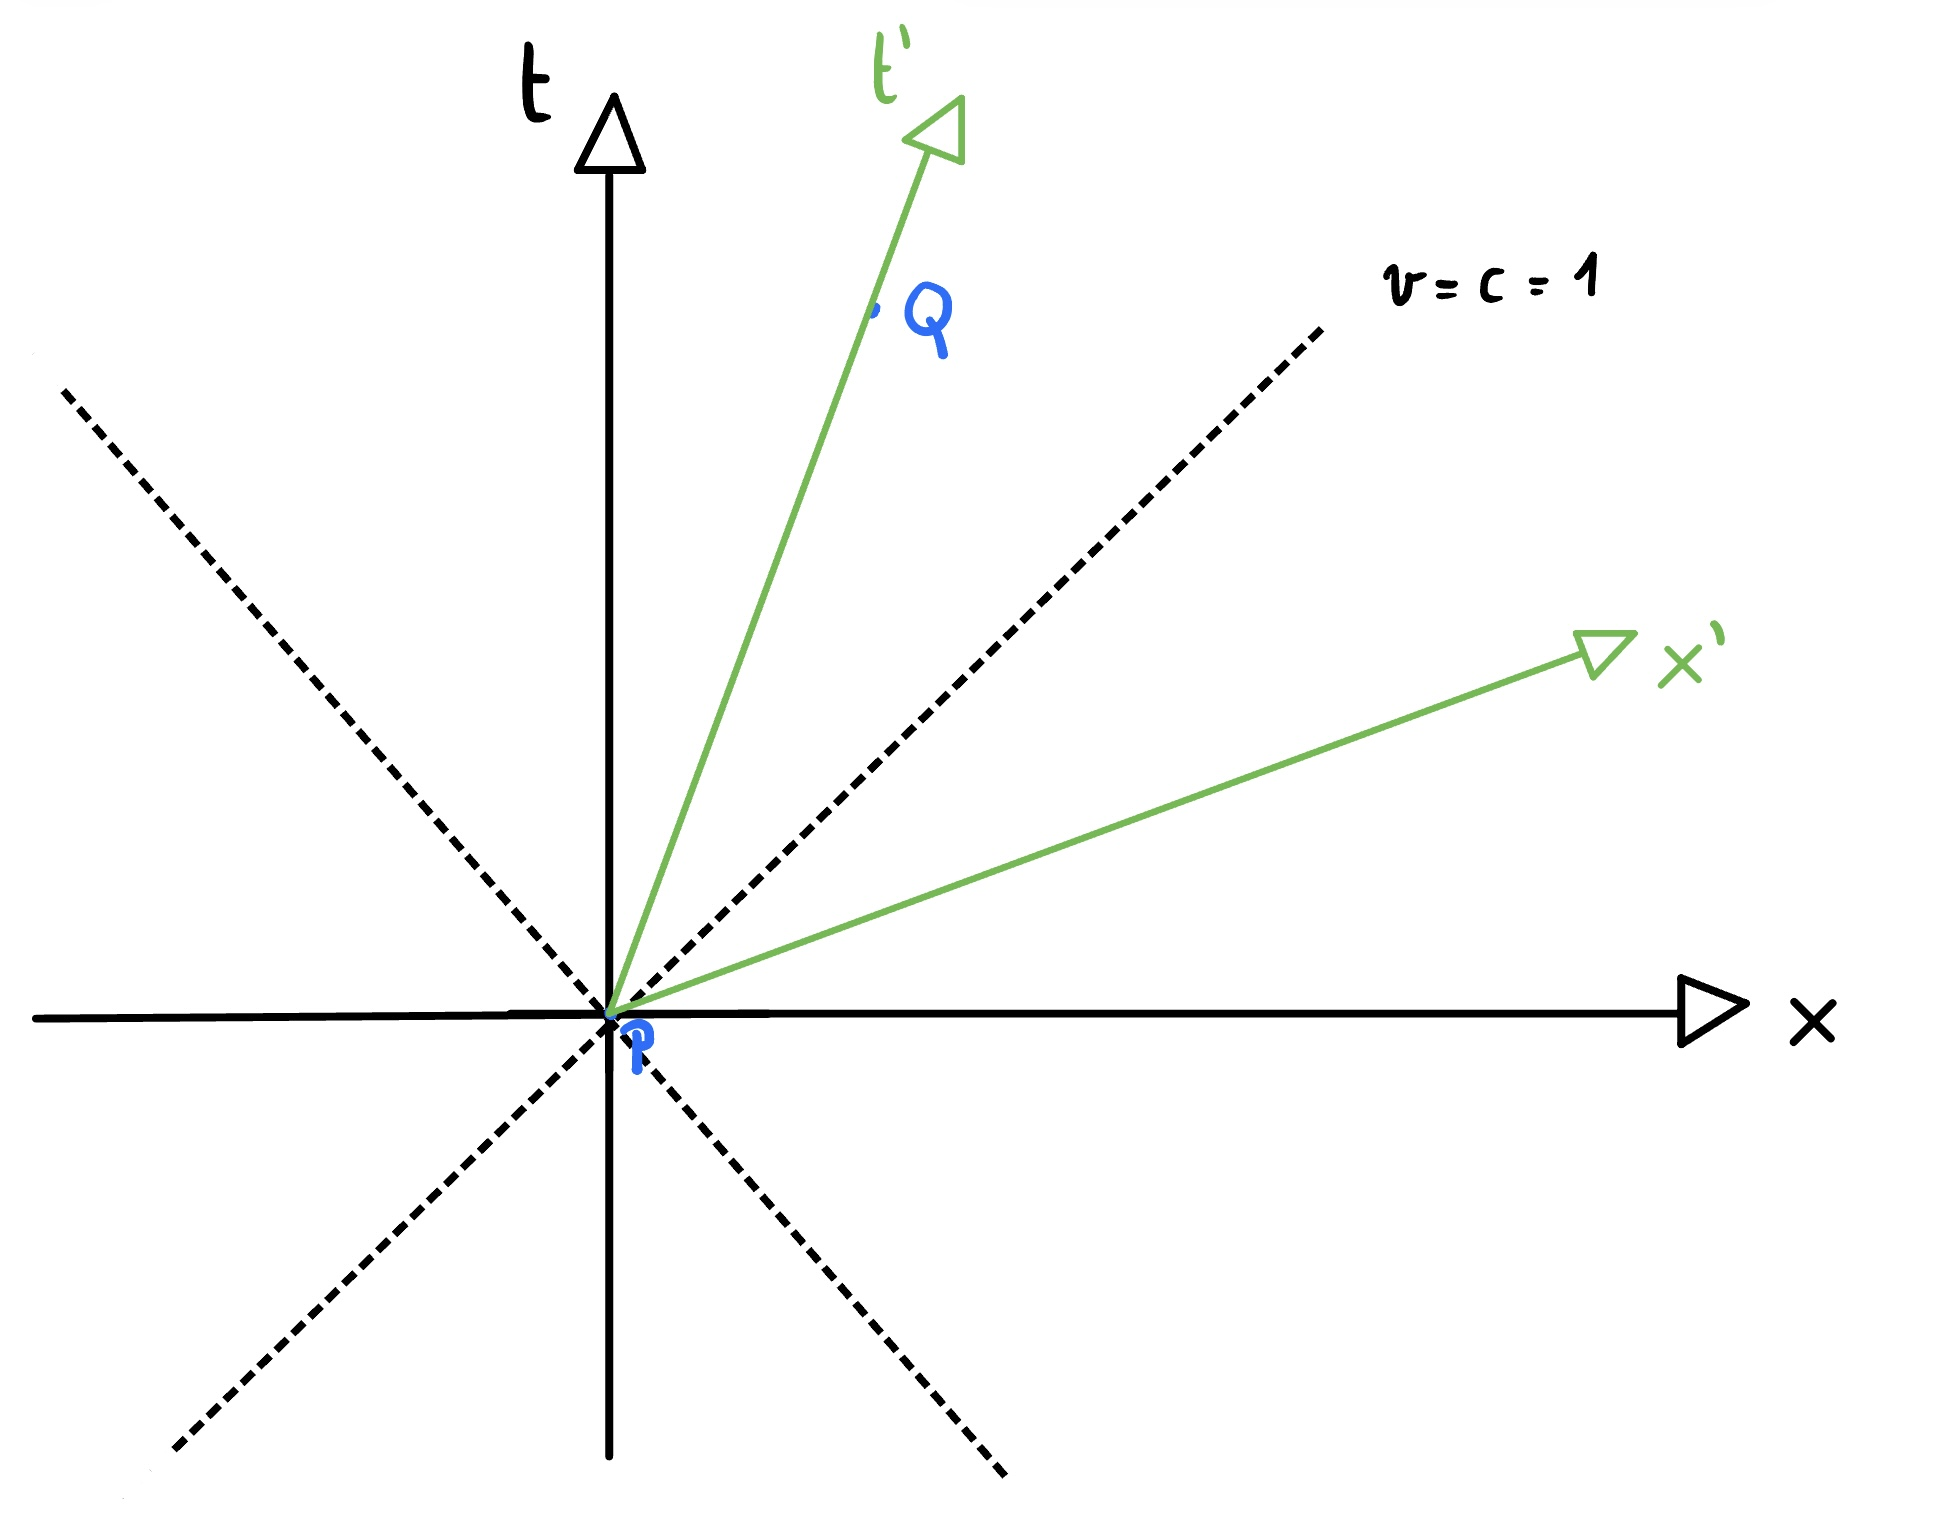
\includegraphics[scale=0.1]{Chapitres/2. Relativité Restreinte/Images/Changement de variable.jpg}
        \caption{Il existe un référentiel tel que deux points causalements connectés se passent au même endroit.}
        \label{fig:2.2}
    \end{center}
\end{figure}

\begin{theoremframe}
    \begin{propri}
        Si $Q$ appartient à l'ailleurs absolu de $P$, alors
        \begin{itemize}
            \item[\emph{(i).}] Il n'existe pas de référentiel inertiel tel que $Q$ se passe au même endroit que $P$.
            \item[\emph{(ii).}] Il est possible de trouver des référentiels inertiels tels que $Q$ se passe avant, en même temps ou après $P$.
        \end{itemize}
    \end{propri}
\end{theoremframe}
\begin{proof}
    Exercice.
\end{proof}

    Comme $Q$ n'est pas dans le cône de lumière, $P$ et $Q$ ne peuvent pas être en contact causal. On peut effectuer un boost tel que deux événements $P$ et $Q$ ont lieu en même temps ( c'est-à-dire que $\Delta t' = 0$). 

    Les cônes de lumière donnent à l'espace-temps de Minkowski une structure très différentes de l'espace-temps euclidien usuel de la théorie de Newton. Dans cette dernière, il n'y a pas de transformation mélangeant espace et temps , et il existe une division logique de l'espace-temps en "tranches ", représentant tout l'espace à un temps donné. En particulier:
    \begin{enumerate}
        \item la notation de simultanéité est absolue (non-ambiguë).
        \item les trajectoires d'une particule sont contraintes uniquement par $\Delta t> 0$. On peut avoir $v>c$
    \end{enumerate}
    En relativité restreinte, la notion de simultanéité devient relative au référentiel choisi et d'autre part, l'espace-temps est structuré par les cônes de lumières en tout point qui déterminent les trajectoires possibles des particules. Par l'invariance de $c$ pour tout référentiel inertiel, on peut déduire que les cônes de lumières sont les mêmes pour tout référentiel inertiel.
    \begin{figure}[H]
        \centering
        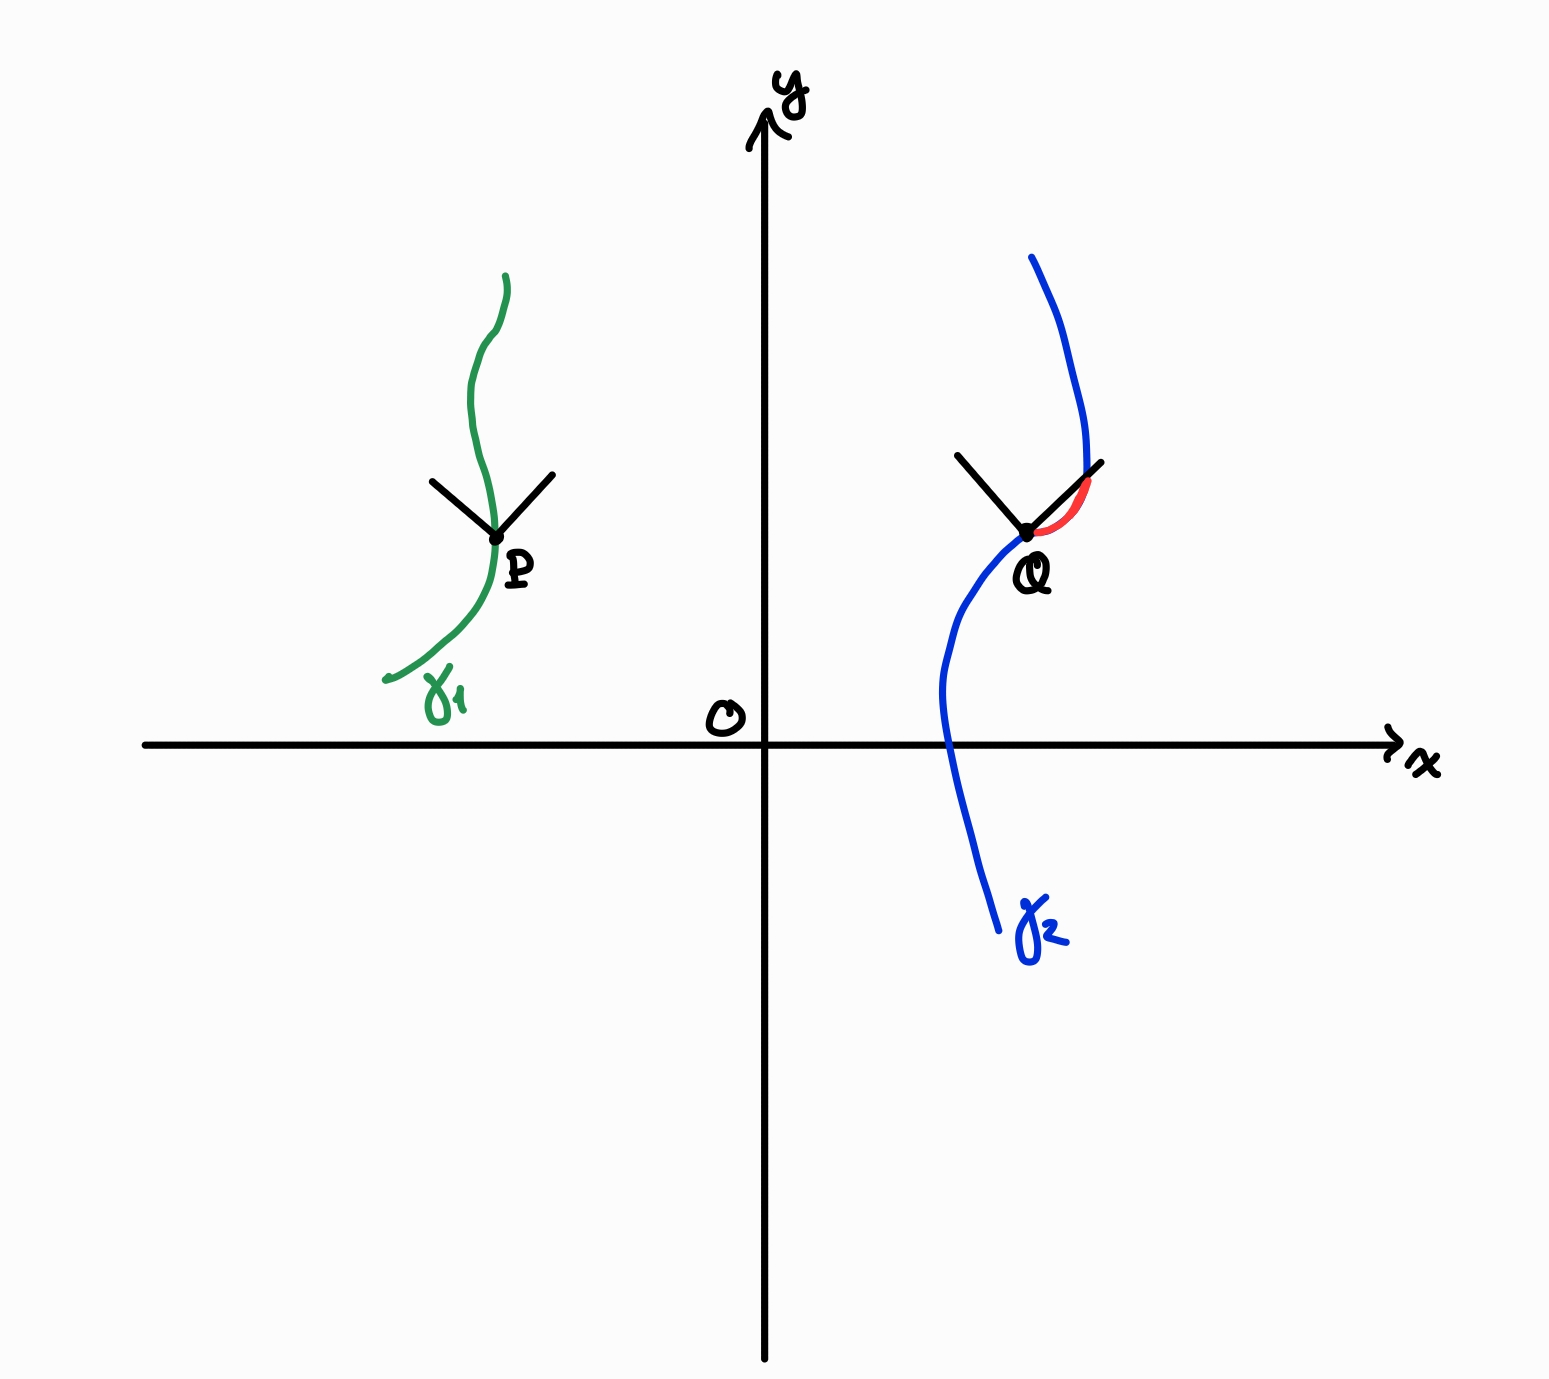
\includegraphics[width=0.5\linewidth]{Chapitres/2. Relativité Restreinte/Images/Courbes non causales.png}
        \caption{En $\R^{1,3}$, uniquement les trajectoires du type $\gamma_1$ sont admissibles. La courbe $\gamma_2$ ne peut pas représenter la trajectoire d'une particule car son tracé n'est plus contenu dans le cône de lumière de $Q$.}
        \label{fig:2.3}
    \end{figure}
\subsection{Temps propre}

Soient deux évènements $P$ et $Q$ causalement liés. 
\begin{theoremframe}
    \begin{defi}
        Le temps propre séparant $P$ et $Q$ est défini comme:
        \begin{equation}
            (\Delta s)^2_{PQ} = -(\Delta \tau)^2
        \end{equation}
    \end{defi}
\end{theoremframe}

Si $P$ et $Q$ représentent une particule libre à des temps différents, le temps propre $\Delta \tau $ est le temps écoulé entre deux évènements pour un observateur attaché au mouvement. En effet, comme les évènements sont causalement liés, il existe un référentiel dans lequel $P$ et $Q$ se passent au même endroit, et donc $(\Delta s)^2=-(\Delta t')^2 =$ et donc $\Delta t' = \Delta \tau$ dans ce référentiel.

\subsection{Courbes causales}
Rappelons la notion de courbe.
\begin{theoremframe}
    \begin{rap}
        Soit $I$, un ouvert de $\R$. Une application (lisse) $\R \to \mathcal{M}: \lambda \mapsto x^\mu (\lambda)$ est appelé courbe (lisse) sur $\mathcal{M}$. Le champ de vecteur tangent à la courbe $v$ est défini par
        \begin{equation}
            v^\alpha = \frac{\td x^\alpha}{\td \lambda}
        \end{equation}
    \end{rap}
\end{theoremframe}
La courbe est dite de genre $\left\{
\begin{array}{l}
 \text{temps} \\
 \text{espace}\\
 \text{lumière}
\end{array}
\right.$
si la norme du champ $ v^2 = v_{\alpha}v^{\alpha}$ 
$\left\{
\begin{array}{l}
 < 0 \\
 > 0\\
 = 0
\end{array}
\right.$
\\
\begin{exmp}
    La norme du vecteur $v = (1,0,0,0)$ est donnée par $\eta_{\alpha \beta}v^{\alpha} v^{\beta} = (-1)v^{0} v^{0} =-1$. La norme n'est donc pas définie positive (comme dans le cas euclidien).
\end{exmp}
\begin{theoremframe}
    \begin{defi}
        Une courbe est dite causale si à tout point de la courbe, le vecteur tangent est
        \begin{itemize}
            \item[(i).] de genre temps ou lumière.
            \item[(ii).] orienté vers le futur ($\frac{\td x^0}{\td\lambda}>0$).
        \end{itemize}
    \end{defi}
\end{theoremframe}
\subsection{Longueur Minkowski d'une courbe causale}

D'après la définition du temps propre de deux évènements causalement liés
\begin{equation}
    \label{eq:temps propre}
   (\Delta \tau)^{2} = -(\Delta s)^2 = (\Delta t)^2 - \sum_{i}(\Delta x^{i})^2 
\end{equation}

on définit le temps propre infinitésimal
\begin{equation}
    d\tau ^2 = -ds^{2} = dt^2 - \sum_{i} (dx^{i})^2
\end{equation}
\begin{figure}
    \centering
    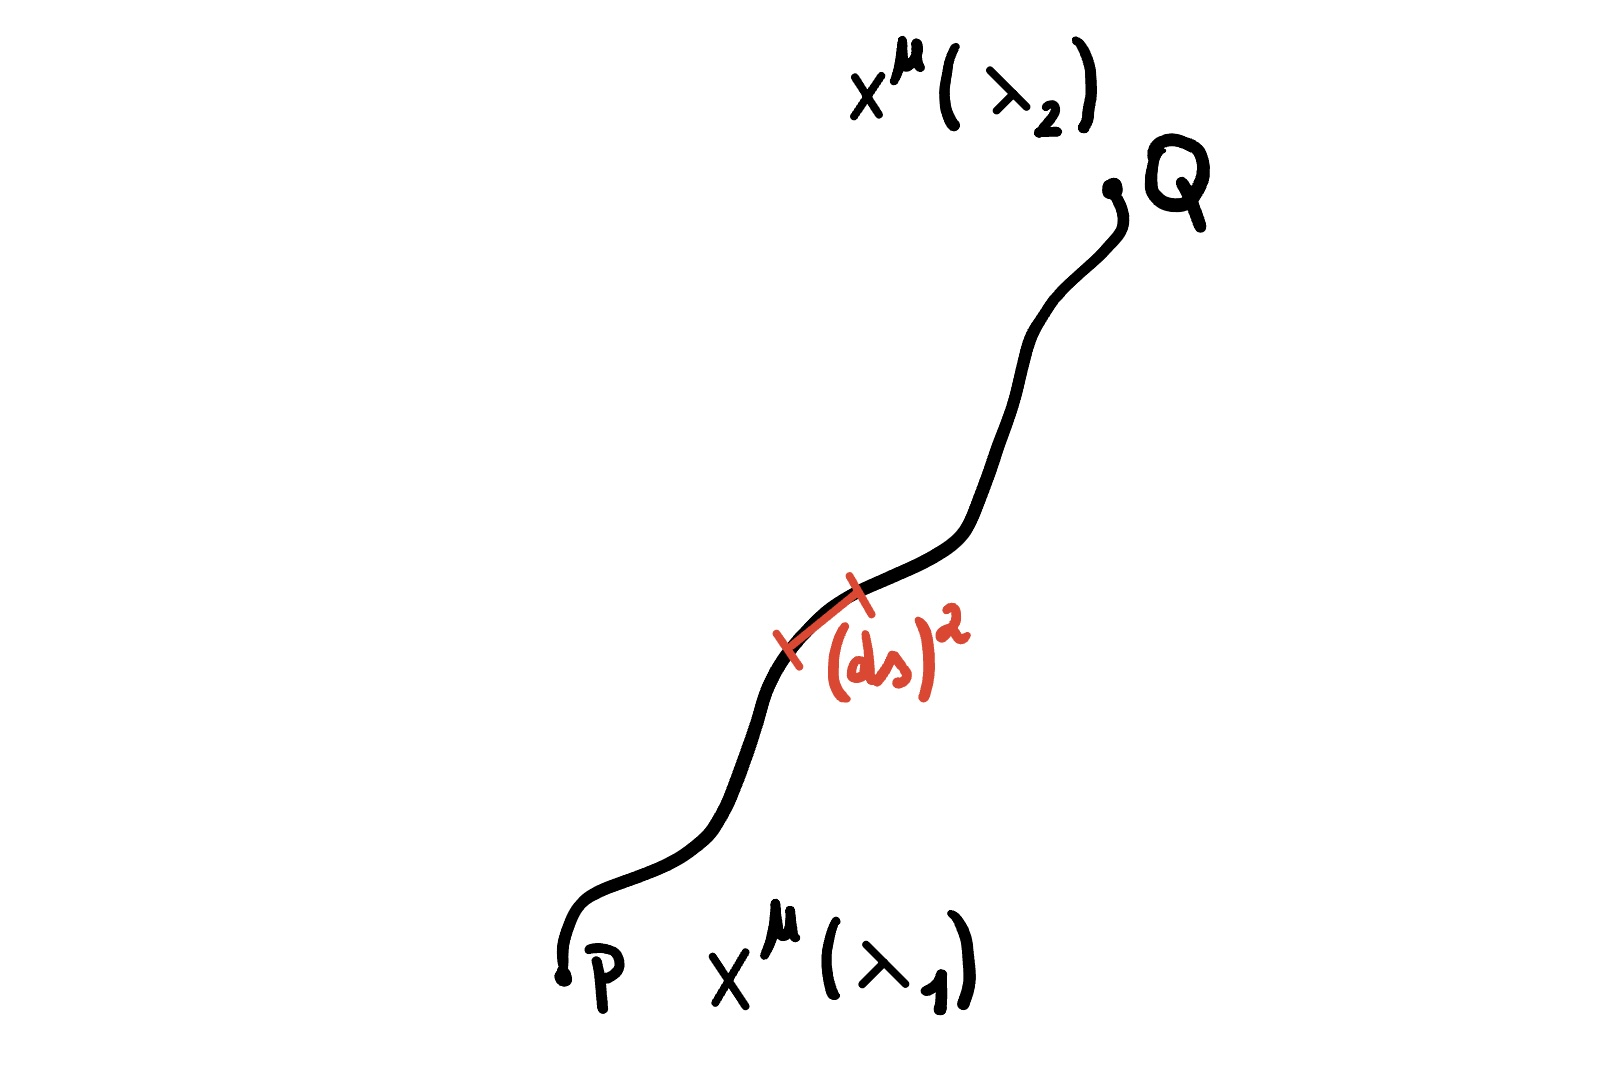
\includegraphics[width=0.5\linewidth]{Chapitres/2. Relativité Restreinte/Images/Coubre.jpg}
    \caption{}
    \label{fig:2.4}
\end{figure}

Cette définition permet nous permet de définir le temps propre d'une courbe causale $\gamma$ arbitraire comme

\begin{align}
    \tau_\gamma &= \int_{\gamma} \td\tau\\
    &= \int^{\lambda_{2}}_{\lambda_{1}}\left(\frac{\td\tau}{\td\lambda}\right)\td\lambda\\
    &= \int^{\lambda_{2}}_{\lambda_{1}} \td \lambda\sqrt{\left(\frac{\td t}{\td\lambda}\right)^2 - \sum_{i}\left(\frac{\td x^{i}}{\td\lambda}\right)^2} 
\end{align}

Et est le temps mesuré par un observateur qui suit la trajectoire. 
\begin{theoremframe}
    \begin{propri}
        Le temps propre entre deux évènements causalement reliés défini par \ref{eq:temps propre} correspond au temps propre de la droite reliant les deux évènements. De plus, la courbe qui maximise le temps propre entre deux évènements est la droite.
    \end{propri}
\end{theoremframe}
\begin{proof}
    Exercice.
\end{proof}
En effet, le temps propre de deux courbes causales distinctes reliant deux évènements n'est en général pas identique. Un exemple de cette propriété est le paradoxe des jumeaux.

\begin{exmp}[Paradoxe des jumeaux\footnote{Disclaimer: il s'agit d'une expérience de pensée. Aucune fusée n'a été blessée au cours de cette expérience.}]
    Supposons que deux jumeaux sur Terre possèdent chacun·es une horloge atomique qui affiche la même heure. Posons leur genre = M. L'un des jumeaux est envoyé dans l'espace à une vitesse proche de celle de la lumière avec cette horloge. Quand il revient sur Terre, en comparant les deux horloges, le jumeaux étant resté sur terre est plus jeune que celui parti dans l'espace. 
\end{exmp}
Pour expliquer ce "paradoxe" (ce n'en est pas réellement un\footnote{En fait, si, selon la définition. \href{https://www.youtube.com/watch?v=ppX7Qjbe6BM}{Vidéo intéressante sur le sujet}.}), intéressons-nous à la situation simplifiée suivante, où un jumeau passe directement de $A$ à $C$, et l'autre jumeau fait un détour par $B'$.
\begin{figure}[H]
    \centering
    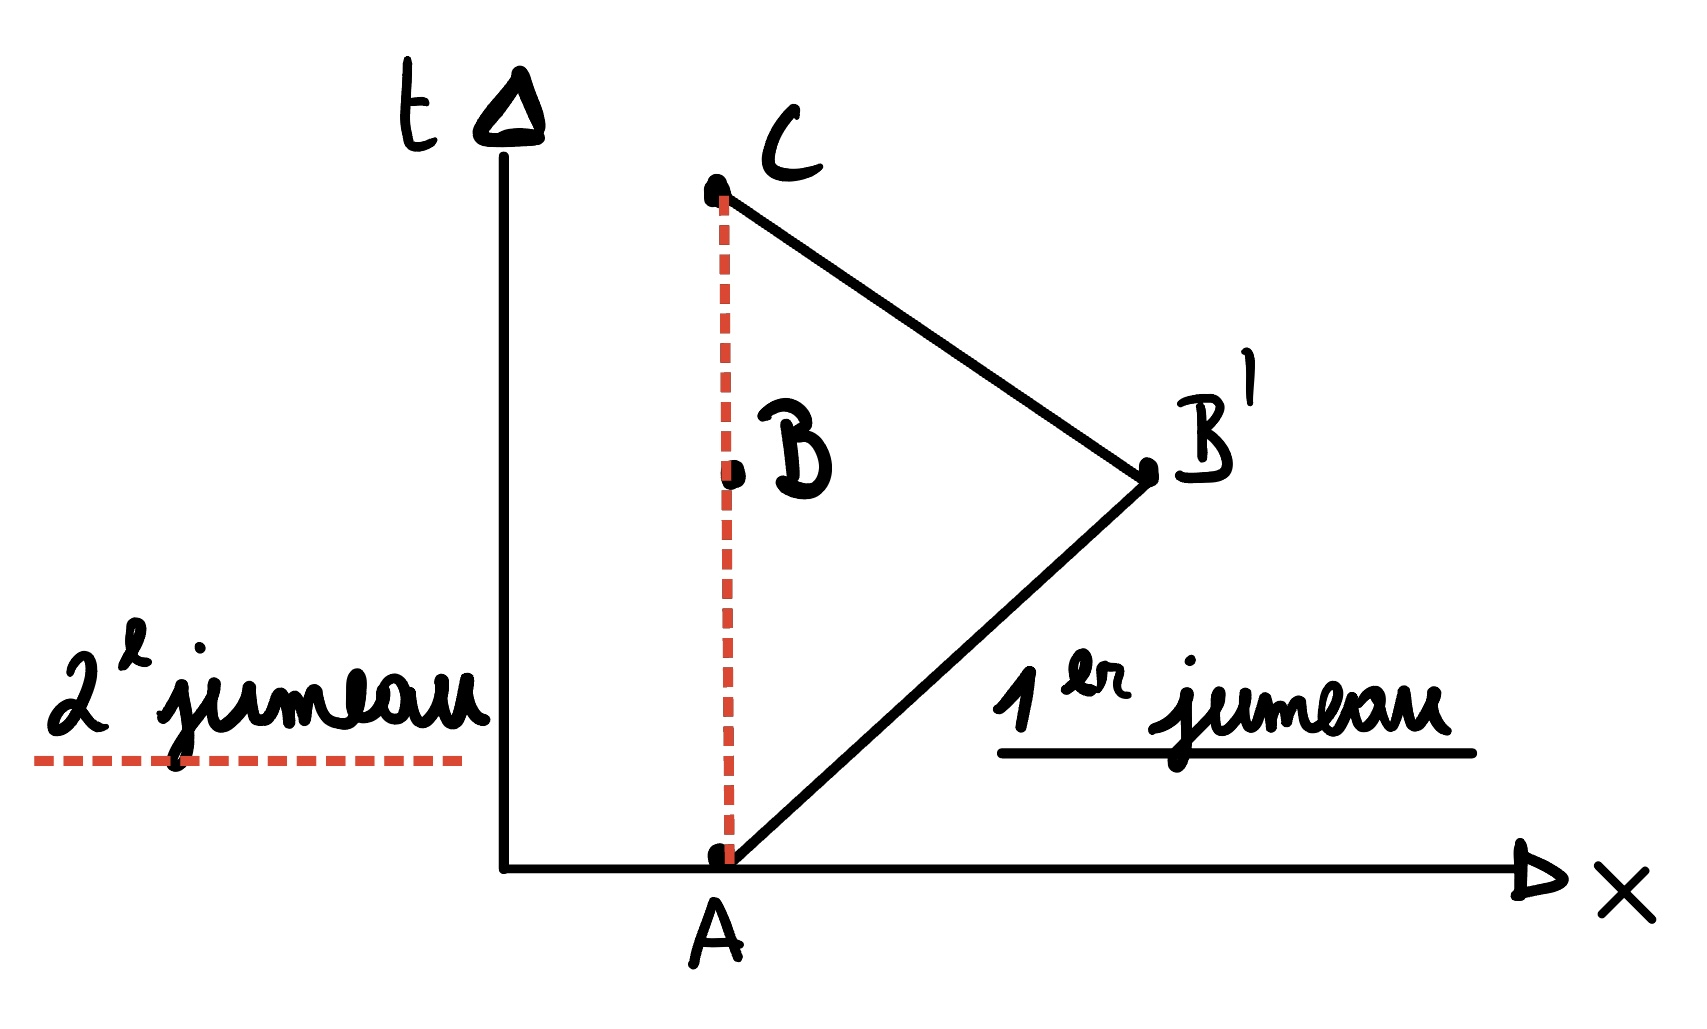
\includegraphics[width=0.5\linewidth]{Chapitres/2. Relativité Restreinte/Images/Deux jumeaux.jpg}
    \caption{}
    \label{fig:2.5}
\end{figure}

Calculons le temps propre des deux chemins. Dans le référentiel $O$, on a pour le deuxième jumeau
\begin{equation}
    (\Delta \tau_{ABC})^2 = (\Delta t)^2
\end{equation} 
Alors que comme $B'=(\frac{\Delta t}{2},\Delta x)$,

\begin{align}
        (\Delta \tau_{AB'C})^2 &= (\Delta \tau_{AB'} + \Delta \tau_{B'C})^2\\
        &= 4(\Delta \tau_{AB'})\\
        &= 4 \left(\left(\frac{\Delta t}{2}\right)^2 - (\Delta x)^2\right)\\
        &= 4 \left(\left(\frac{\Delta t^2}{4}\right) - (\Delta x)^2\right)
    \end{align}
    On peut définir $v = \dfrac{\Delta x}{(\Delta t/2)} = \dfrac{2 \Delta x}{\Delta t}$ qui est tel que $v^2 = \frac{4(\Delta x)^2}{(\Delta t)^2}$ et donc
    \begin{align*}
        (\Delta \tau_{AB'C})^2 &= (\Delta t)^2(1 - v^2)\\
        &< (\Delta t)^2
    \end{align*}

Le temps propre du premier jumeaux (voyageur) est plus petit que le temps propres du jumeau 2 (au repos). 
\begin{center}
    \textit{Le temps s'écoule plus lentement quand on est en mouvement.}
\end{center}

\subsection{Horizon des événements} 

Soit $\mathcal{S} \in \R^{1,3}$  un sous-ensemble de Minkowski. 
\begin{theoremframe}
    \begin{defi}
        Le futur chronologique $I^{+}(\mathcal{S})$ est l'ensemble des points de $\R^{1,3}$ qui sont reliés à un point de $\mathcal{S}$ par une courbe causale de genre temps. 
    \end{defi}
\end{theoremframe}
\begin{theoremframe}
    \begin{defi}
        Le futur causal $J^{+}(\mathcal{S})$ est l'union de $\mathcal{S}$ avec tous les points de $\R^{1,3}$ qui sont reliés à un point de $\mathcal{S}$ par une courbe causale. 
    \end{defi}
\end{theoremframe}

\begin{exmp}
    Si $\mathcal{S} = \{P\}$ alors $I^{+}(\mathcal{S}) = \mathrm{int}( C_{P}^{+})$ et $J^{+}(\mathcal{S}) = C_{P}^{+} \cup \{P\}$. 
\begin{figure}[H]
    \centering
    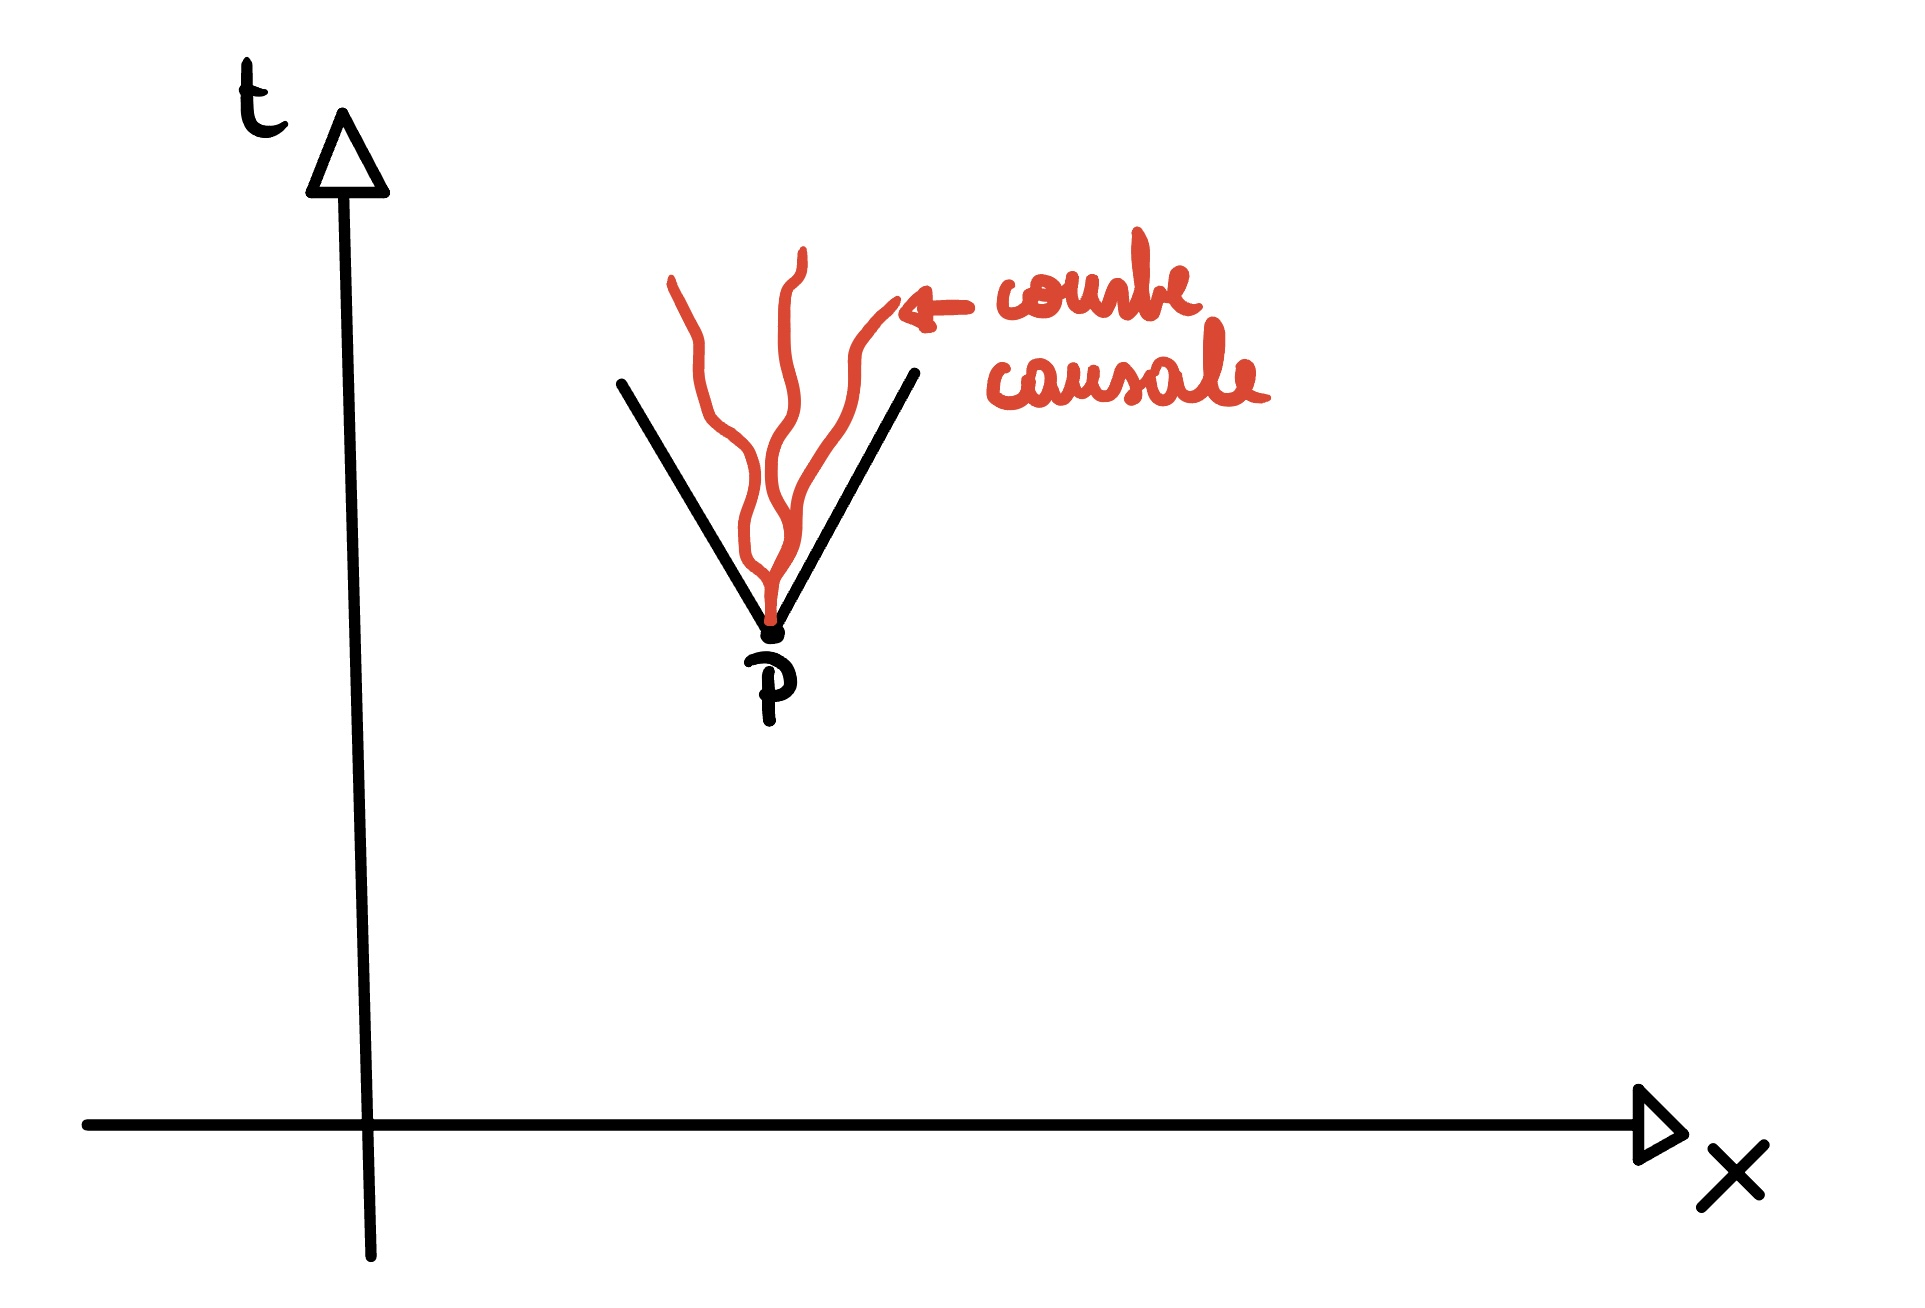
\includegraphics[width=0.5\linewidth]{Chapitres/2. Relativité Restreinte/Images/exemple1.jpg}
    \caption{}
    \label{fig:2.6}
\end{figure}
\end{exmp}

    \begin{exmp}
    Si $\mathcal{S}$ est la trajectoire d'un observateur inertiel au repos, alors $I^{+}(\mathcal{S}) = J^{+}(\mathcal{S}) = \R^{1,3}$ tout entier.
    \begin{figure}[H]
        \centering
        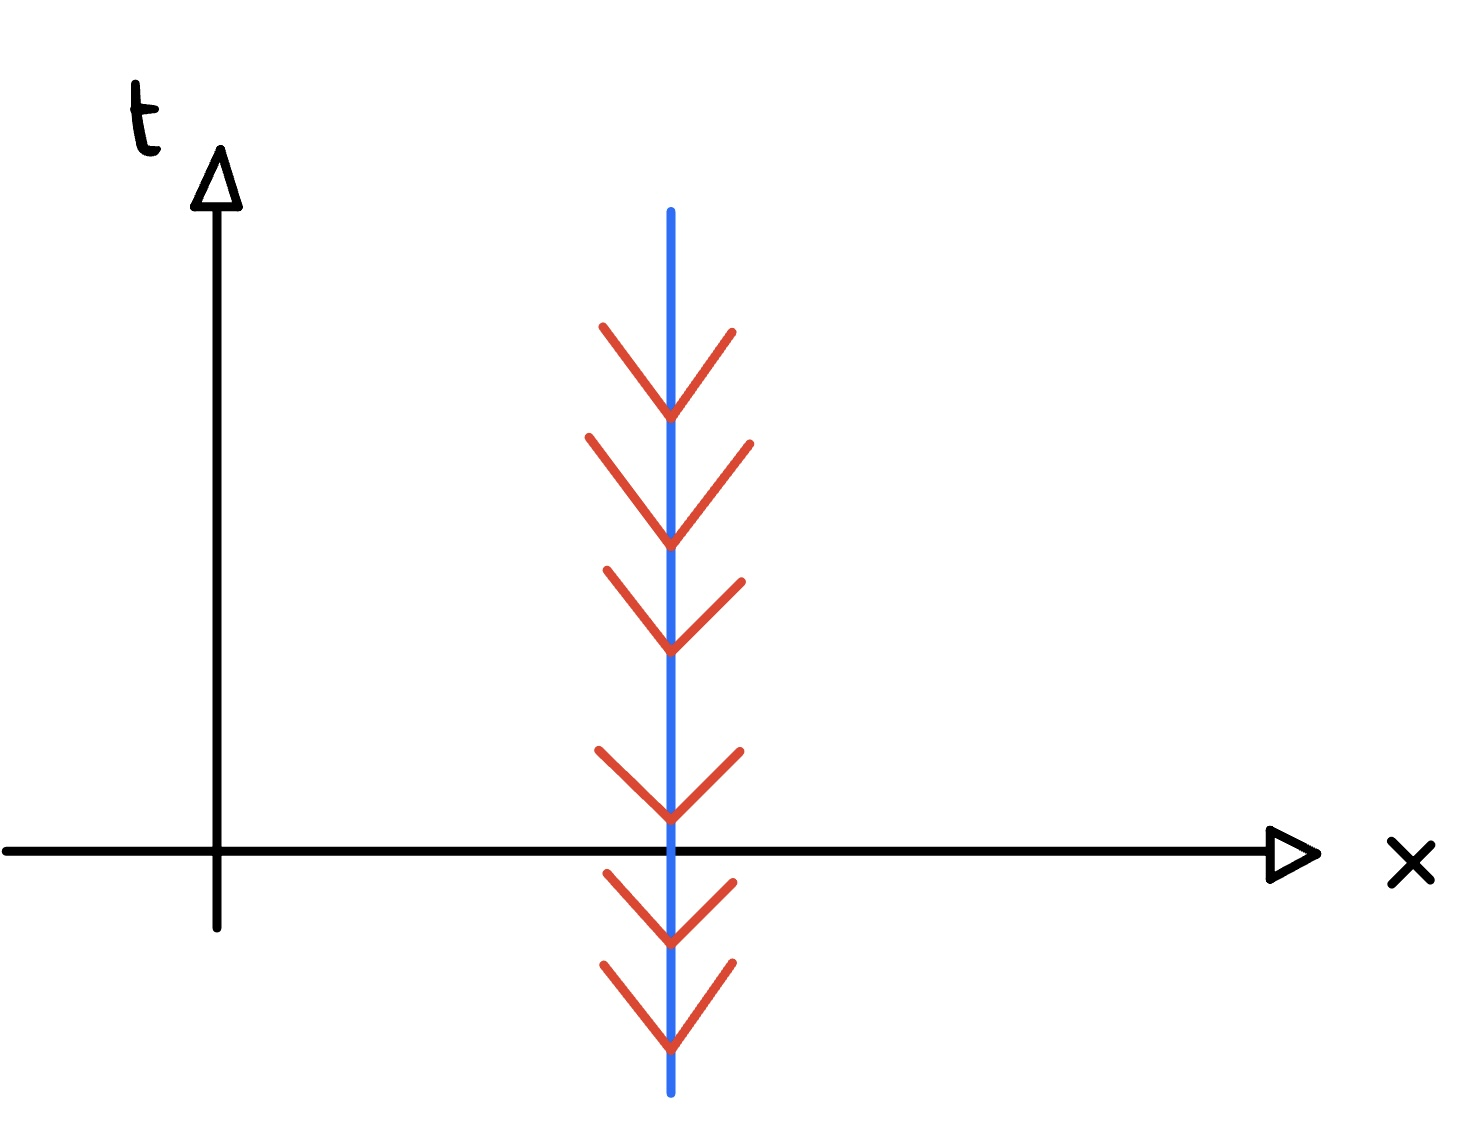
\includegraphics[width=0.5\linewidth]{Chapitres/2. Relativité Restreinte/Images/exemple2.jpg}
        \caption{}
        \label{fig:2.7}
    \end{figure}
\end{exmp}
\begin{exmp}[Expérience de Rindler\footnote{Attention aux débutant·es, il s'agit de nouveau d'une expérience de pensée !}]
    Considérons maintenant le cas d'un observateur accéléré. Soit $x^{\alpha}(\lambda)$, une courbe de genre temps. Alors
    
    \begin{equation}
    \eta_{\alpha \beta} \frac{\td x^{\alpha}}{\td \lambda}\frac{\td x^{\beta}}{\td \lambda} = -\alpha^2(\lambda) < 0
    \end{equation}

    On souhaite effectuer un changement de variable $\lambda \to \mu$ tel que $\alpha(\mu) = 1$.

    \begin{equation*}
        \eta_{\alpha \beta} \frac{\td x^{\alpha}}{\td \mu}\frac{\td x^{\beta}}{\td \mu} \left(\frac{\td \mu}{\td \lambda}\right)^2 = -\alpha(\lambda)^2
    \end{equation*}

    Ainsi, on peut choisir $ \mu (\lambda )$ tel que $\left(\dfrac{\td \mu}{\td \lambda}\right)^2 = \alpha(\lambda)^2$.

    Ce qui implique que: 

    \begin{equation*}
         \eta_{\alpha \beta} \frac{\td x^{\alpha}}{\td \mu}\frac{\td x^{\beta}}{\td \mu} = -1
    \end{equation*}
    On peut écrire $\mu (\lambda )$ de manière infinitésimal tel que $-d\mu ^2 = \eta_{\alpha \beta} \td x^{\alpha} \td x^{\beta} = \td s^2 = -d\tau^2$ et donc $x^{\alpha}(\mu) = x^{\alpha}(\tau)$, soit

    \begin{equation*}
        \eta_{\alpha \beta} \frac{\td x^{\alpha}}{\td \tau}\frac{\td x^{\beta}}{d \tau} = -1
    \end{equation*}

    La 4-vitesse le long d'une courbe est définie par:

    \begin{equation*}
        v^{\alpha} = \frac{\td x^{\alpha}}{\td \mu}
    \end{equation*}

    où $v^{\alpha} v_{\alpha} = -1$.

    La 4-accélération est définit par: 

     \begin{equation*}
        a^{\alpha} = \frac{\td v^{\alpha}}{\td \mu}
    \end{equation*}
    Nous souhaitons étudier la trajectoire d'un observateur à accélération constante, qui est un observateur tel que: 
    \begin{equation*}
        a_{\alpha}a^{\alpha} = a^{2} = \text{cste}
    \end{equation*}
    Choisissons un référentiel tel que l'accélération se fait dans la direction $x^{1}$ et décrit un mouvement dans le plan $(x^{0}, x^{1})$. Nous supposerons que $v^2 = v^3 = 0$. Les équations du mouvement pour cet observateur accéléré sont
\begin{align}
  \dfrac{d x^{\alpha}}{d \tau} = v ^{\alpha}\\
 \dfrac{d v^{\alpha}}{d \tau} = a^{\alpha}
\end{align}
muni des conditions
\begin{align}
    v^{\alpha}v_{\alpha} & = -1 = -(v^{0})^2 + (v^{1})^2\\
    a^{\alpha}a_{\alpha} & = a^2 = -(a^{0})^2 + (a^{1})^2 = \mathrm{cste}
\end{align}

Or, comme $v^{\alpha}v_{\alpha} = -1$:

\begin{align}
    \frac{\td v^\alpha v_\alpha}{\td \tau} &= 2 a^{\alpha}v^{\alpha} = 0 \\
    \implies &-a^{0}v^{0} + a^{1}v^{1} = 0\\
    \label{eq:2.57}
    \implies &v^{1} = \frac{v^{0}a^{0}}{v^{1}}
\end{align}

En adoptant temporairement des indices covariants purement pour question de visibilité:

\begin{align}
    a_1^2 &= 1 \cdot a_1^2\\
    &= \lt v_0^2 - v_{1}^2 \rt a_{1}^2\\
    &= v_{0}^2 \lt 1 - \frac{a_0^2}{a_1^2} \rt a_1^2\\
    &= v_{0}^2(a_{1}^2 - a_{0}^2)\\
    &= v_{0}^2 a^2
\end{align}

Nous obtenons donc que $a^1 = av^{0}$ et que $a^0 = av^{1}$ par \ref{eq:2.57}. Ce problème peut se réécrire en forme matricielle comme:
\begin{equation}
\frac{\td }{\td \tau} \begin{pmatrix}
    v^0 \\
    v^1
\end{pmatrix} = \begin{pmatrix}
    0 & a \\
    a & 0
\end{pmatrix}
\begin{pmatrix}
    v^0 \\
    v^1
\end{pmatrix}
\end{equation} 

La solution de ce système est

$\Rightarrow $\begin{equation*} \left\{
\begin{array}{l}
  v^{0} = \cosh{a\tau}\\
 v^{1} = \sinh{a\tau}\\
\end{array}
\right.
\end{equation*}

Et la position est donc donné par

$\Rightarrow $\begin{equation*} \left\{
\begin{array}{l}
  x^{0} = \frac{1}{a}\sinh{a\tau}\\
 x^{1} = \frac{1}{a}\cosh{a\tau}\\
\end{array}
\right.
\end{equation*}

À quoi ressemble cette trajectoire graphiquement ? On a que:

\begin{align*}
    &v^{1} = 0|_{\tau = 0}\\
    &(x^1)^2 - (x^0)^2 = \frac{1}{a^2}
\end{align*}

il s'agit donc d'une branche d'hyperbole.
\begin{figure}[H]
    \centering
    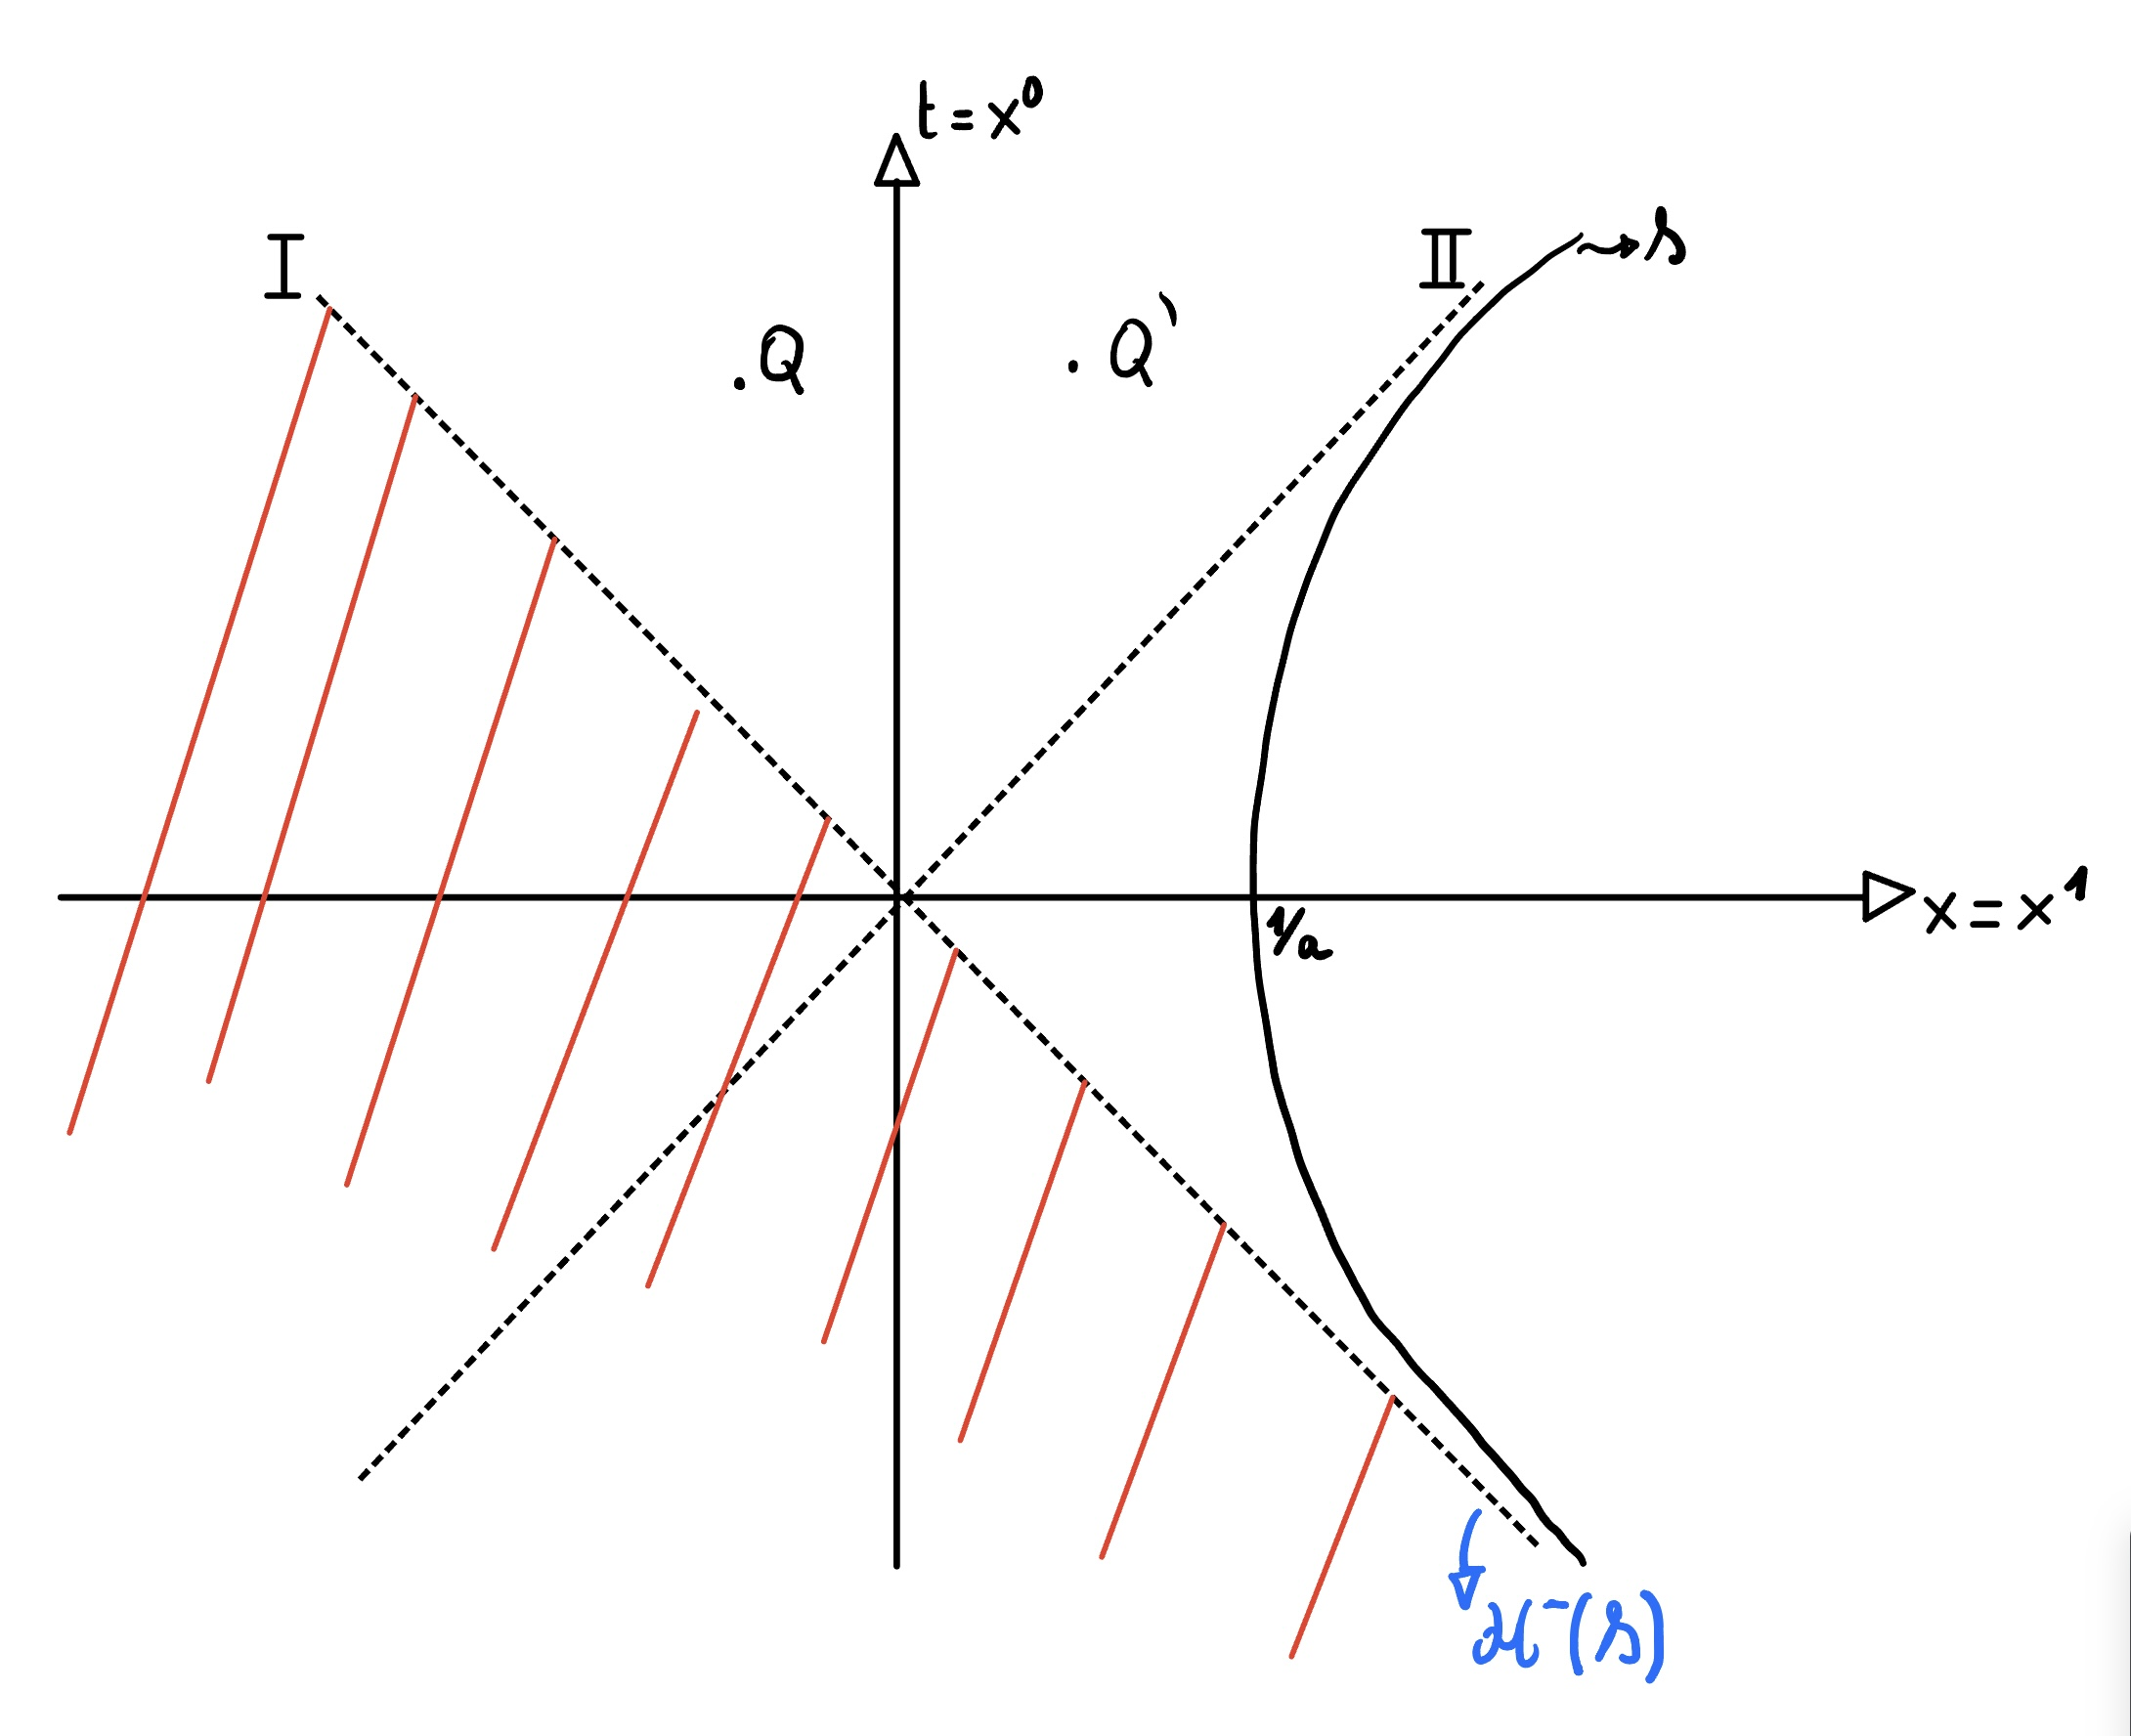
\includegraphics[width=0.5\linewidth]{Chapitres/2. Relativité Restreinte/Images/Courbe hyperbole 1.jpg}
    \caption{}
    \label{fig:2.8}
\end{figure}

Cette ensemble de points $\mathcal{S}$ est la trajectoire d'un observateur accéléré dans l'espace-temps de Minkowski. Quelques remarques:
\begin{enumerate}
    \item $\mathcal{S}$ ne pourra jamais influencer ce qui se trouve sous la ligne de lumière \cRM{1} (indiqué en rouge sur la figure \ref{fig:2.8}). 

    \item $I^{+}(\mathcal{S})$ est l'ensemble des évènements que la trajectoire $\mathcal{S}$ peut influencer, et correspond à la zone non hachurée de la figure \ref{fig:2.8}.

    \item La frontière de $I^{+}(\mathcal{S})$ est l'horizon des événements passé de $\mathcal{S}$. $\mathcal{H}^{+}(\mathcal{S}) = \cRM{1}$ est la frontiére de l'horizon des événements passé. 
\end{enumerate}



La frontière de $\cRM{1}^{+}(\mathcal{S})$ est l'horizon des événements passé de $\mathcal{S}$. $\mathcal{H}^{+}(\mathcal{S}) = \cRM{1}$ est la frontiére de l'horizon des événements passé. 

\begin{center}
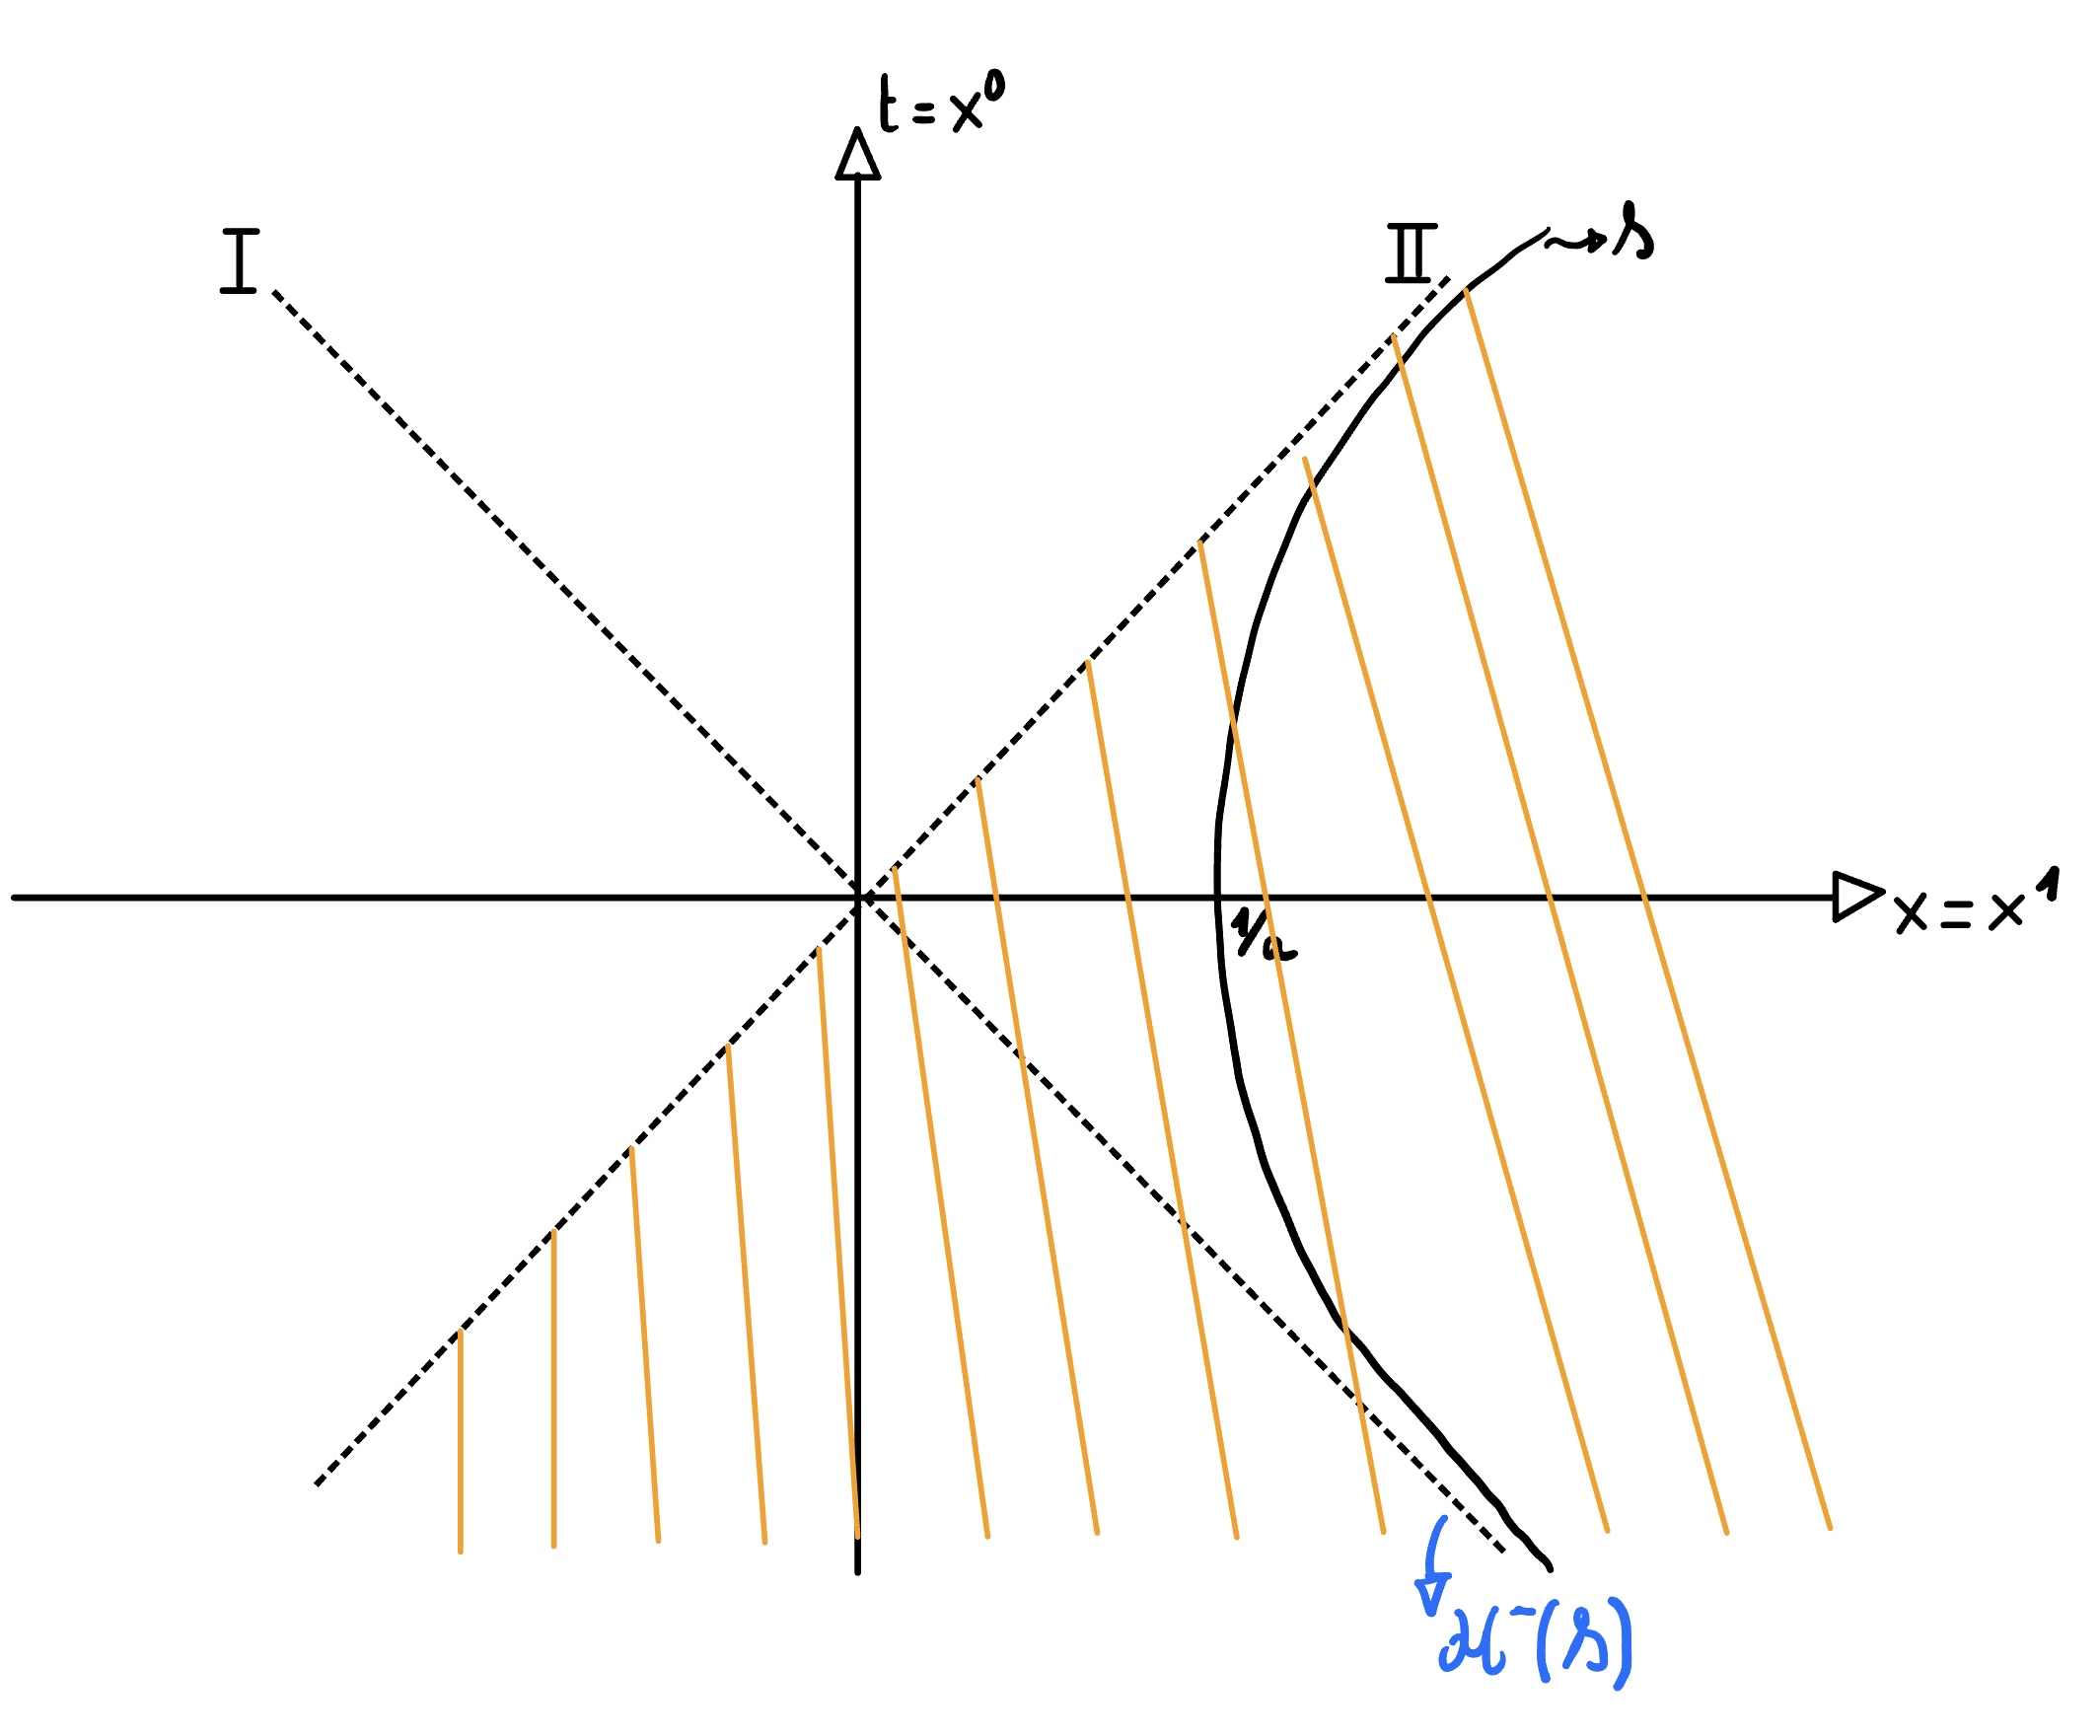
\includegraphics[scale=0.1]{Chapitres/2. Relativité Restreinte/Images/Courbe hyperbole 2.jpg}
\label{Parabolique 2}
\end{center}

$\cRM{1}^{-}(\mathcal{S})$ est une zone où la trajectoire $\mathcal{S}$ peut être affecté par les événements qui ont lieu dans la zone hachurée pour la graphique \ref{Parabolique 2}. 

La frontière de $\cRM{1}^{-}(\mathcal{S})$ est l'horizon des événements futur  de $\mathcal{S}$. Qu'on note $\mathcal{H}^{-}(\mathcal{S})$.

\end{exmp}

\section{Hypersurfaces de Cauchy}
La notion d'hypersurface de Cauchy est importante afin que les problèmes aux limites est bien posé\footnote{Selon Hadamard :)}.

\begin{theoremframe}
    \begin{defi}
        Le \textit{domaine de dépendance future} (ou \textit{développement futur}) d'une région $\mathcal{S}$ de l'espace-temps est l'ensemble des points $P \in \R^{1,3}$ tels que toute courbe causale passant par $P$ intersecte $\mathcal{S}$. Il est noté $\mathcal{D}^+(\mathcal{S})$.
    \end{defi}
\end{theoremframe}
\begin{exmp}
    Soit ???? wtf ?????
\end{exmp}










